%-------------------------------------------------------%
%                        第4章实例
%-------------------------------------------------------%
% \chapter{基于改进的MAPPO算法的常规公交驻站控制}\label{第4章}
\chapter{基于改进MAPPO的公交驻站防串车控制算例仿真与实例分析}\label{第4章}
% 为了验证本文提出的基于改进的MAPPO强化学习算法的公交驻站控制策略的现实可行性，
% 本章将模型的应用场景由第3章提出的单向环形公交线路拓展真实的常规公交线路中。

为验证本文提出的基于改进多智能体近端策略优化（改进MAPPO）算法的公交驻站防串车控制方法的有效性，
本章基于第三章构建的理论框架，通过仿真实验与真实场景验证相结合展开实证分析。
首先，以单线环形公交线路为基准场景，构建高自由度仿真实验环境，验证算法的收敛性与稳定性，
并通过与传统控制策略（基于固定车头时距的控制、基于时刻表的控制、基于前向车头时距的控制、
基于后向车头时距的控制）和基于原始MAPPO算法的控制方法的对比，验证其在均衡车头时距、降低乘客平均等待时间
等方面的性能优势。其次，为进一步验证算法的现实可行性，
将应用场景进一步扩展至真实常规公交线路中，搭建真实场景验证平台，采用多维评价指标体系，
验证其缓解串车现象、减低乘客出行成本方面的显著优势。

本文采用PyCharm搭建仿真实验环境，算法训练采用Python 3.9编程语言和PytTorch 2.0.0深度学习框架实现。
\section{算例分析}
\subsection{实验设置}
% 本文中的实验使用PyCharm搭建模拟环境，算法训练过程使用Python 3.9和PytTorch 2.0.0实现。
本节算例的仿真环境基于一条单向环形公交线路构建，参考Dangzo\cite{daganzo2009headway}和Wang
等人\cite{wang2020dynamic}的设置框架，在环形线路上共设$m=$ 12个均匀分布的公交站点，部署$n=$ 6辆同构运营公交车辆。
公交车辆在站间均以$v=$ 20 km/h的速度匀速运行，相邻辆公交站点间距1 km，
车辆在相邻站点的站间运行时间为3 min（不包括站点乘客的上下车用时和公交的驻站时长）。

系统中每个公交车辆都从起始站点$s_1$按顺序发出，初始发车时间间隔$H=$ 360 s，车辆发出后
沿着线路循环运行，所有车辆在到达的第一个站点，即发车站点$s_1$，不实施驻站控制。
公交车辆的最大载客容量$U=$ 80人。乘客上下车用时参考Chen L等人\cite{chen2016real}的研究设定：
每位乘客的上车时间$t_b=$ 3 s/人，下车时间$t_a=$ 1.8 s/人。
我们与Wang等人\cite{wang2020dynamic}采用相同的设置，将公交在每个站点驻站时间阈值设为
$\triangle T =$ 180 s，当驻站时间低于30 s时忽略不计，视为公交不进行驻站控制干预。

公交系统运行开始后，公交车辆从发车站点沿着环形线路持续循环运行，达到运行周期终止条件时结束运行，
当仿真时间步达到预设阈值时，系统自动终止运行。


仿真环境中每个公交站乘客到达遵循泊松过程，各站点具体到达率分布见下图\ref{fig:乘客到达率}所示\cite{wang2020dynamic}。
乘客的目的站点随机分配为上车站点后方11个站点之一。每个公交站点
积累乘客的时间由相邻车辆到站的时间间隔动态确定，而当公交站点是第一次有公交到站时，其累积乘客的时间
为4 min。
\begin{figure}[!ht]
    \centering
    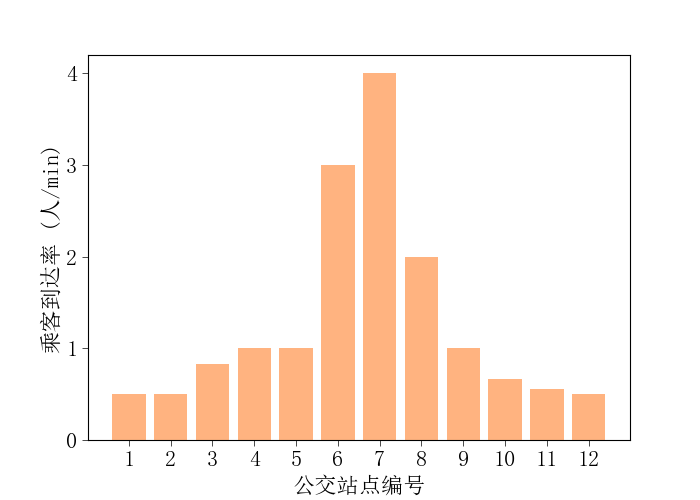
\includegraphics[width=0.67\linewidth]{figures/环形线路公交站点乘客到达率.png}
    \caption{各公交站点乘客到达率}
    \label{fig:乘客到达率}
\end{figure}


\subsection{对比基准模型}

为了全面评估基于改进MAPPO算法的公交驻站控制模型的性能，本节选取六个基准模型进行对比分析，
其中包含基于规则的控制模型（基于固定车头时距、时刻表的控制模型）、传统的数学优化模型（基于
前向车头时距、后向车头时距的控制模型）和基于原始MAPPO强化学习算法的驻站控制模型。

（1）无控制模型（NH）

无控制模型中，不主动实施驻站控制干预，但由于本节提出的公交系统不允许超车，
所以当发生串车时，后面的车辆将被强制驻站。

（2）基于固定车头时距的控制模型（HH）

基于固定车头时距的控制模型是进行简单的控制，当实际车头时距小于计划车头时距时触发驻站，
驻站时长$th=H_0-h^-$，$H_0$是计划车头时距，本文参考Chen W等人\cite{chen2016real}的研究，
将$H_0$设置为360 s。

（3）基于时刻表的控制模型（SH）

基于时刻表驻站的控制模型中，公交车辆的到站时间小于时刻表给定的时间就会触发驻站控制。
在这种情况下，若公交的到站时间大于给定时刻表设定的到站时间，公交在该站点不需要进行
驻站控制，若公交早于给定时刻表的到达站点，要驻站到给定的发车时间时才能离开站点。

（4）基于前向车头时距的控制模型（FH）

Daganzo\cite{daganzo2009headway}2009年提出了基于前向车头时距的控制模型，
驻站时长由下式（\ref{基于前向车头时距的驻站控制}）决定，
\begin{equation}\label{基于前向车头时距的驻站控制}
    th = \max\{ 0,\overline{d}+g(H_0 - h^-) \},
\end{equation}
其中，$H_0$是计划车头时距,$\overline{d} $是平衡时的平均延误，$g>$0是一个控制参数。
我们使用与Daganzo\cite{daganzo2009headway}相同的参数。

（5）基于后向车头时距的控制模型（BH）

采用Xuan等人\cite{xuan2011dynamic}2011年提出基于后向车头时距的控制策略，
驻站时长$th= \beta h^+$，$ h^+$是后向车头时距，$\beta$
是要设置的参数，参考论文中的取值，取0.5。

（6）基于MAPPO算法的驻站控制模型（MAPPO）

原始MAPPO算法模型是未引入图注意力网络（Graph Attention Network, GAT）与异步决策机制的
基线强化学习模型，
为了评估本文所提出的基于改进MAPPO算法模型的性能优势，通过参数一致性设计，
保证两个强化学习模型使用相同的训练参数。


\subsection{评价指标}

参考Berrebi等人\cite{berrebi2018comparing}和Rodriguez\cite{rodriguez2023cooperative}的研究，
从乘客和公交运行商的角度评价公交服务效率和运营可靠性，本文构建了如下四元评价体系：

（1）平均驻站时间（AHT）

平均驻站时间是在模拟运行期间每辆公交车在每个站点的平均驻站时间，该指标反映了驻站控制策略对
公交运行的干预程度与车乘客由于公交驻站增加的额外行程时间。

（2）平均等待时间（AWT）

平均等待时间是在模拟运行期间系统中每位乘客在站点的平均等待时间，该指标可以很好表征
公交的服务响应性和可靠性。

（3）平均旅行时间（ATT）

平均旅行时间是在模拟期间，所有乘客从到达站点等待上车到完成整个行程下车离开站点，整个过程中的平均用时，
该指标能够是综合评估行程效率的全局指标。

（4）平均占用离散度（AOD）

平均占用离散度是每个站点所有公交车辆占用率离散度的均值，车辆占用率的离散度用车上乘客数量的方差
和均值之比表示，该指标通过载客量变异系数量化串车现象，可以用来评价公交服务的可靠性和乘客的出行
乘坐体验，当公交车发生串车时，前车通常会挤满乘客，而后车几乎是空的，公交车辆的载客量
出现高度不均的现象，平均占用离散度（AOD）值会很大，
表达式见下式（\ref{平均占用离散度}）。
\begin{equation}\label{平均占用离散度}
    Var(o_{i,j}) / E(o_{i,j}).
\end{equation}


\subsection{模型训练与收敛性分析}
对本文提出的强化学习模型进行了300轮次训练， 参考Chen等人\cite{chen2016real}和Wang等人\cite{wang2020dynamic}的实验设置，
每轮次包含3 h的完整动态仿真运行，
其中前25 min为预热阶段。
强化学习算法的核心超参数的具体取值见下表\ref{tab3-3}。
\begin{table}[!ht]
\centering
\caption{改进MAPPO算法超参数取值}
\label{tab3-3}
\begin{tabular}{>{\centering\arraybackslash}m{1.8cm} >{\centering\arraybackslash}m{3.8cm} >{\centering\arraybackslash}m{1.8cm} >{\centering\arraybackslash}m{1.8cm}}
\toprule
\textbf{参数类别} & \textbf{参数名称} & \textbf{符号} & \textbf{取值} \\
\midrule
\multirow{3}{*}{优化器} & 策略网络学习率 & $\alpha_{\text{Actor}}$ & 1e-4 \\
    & 价值网络学习率 & $\alpha_{\text{Critic}}$ & 1e-4 \\
    & Adam $\epsilon$参数 & $\epsilon$ & 1e-5 \\
\midrule
\multirow{2}{*}{梯度控制} & Actor梯度裁剪阈值 & $c_{\text{Actor}}$ & 5 \\
    & Critic梯度裁剪阈值 & $c_{\text{Critic}}$ & 5 \\
\midrule
\multirow{5}{*}{强化学习} & 折扣因子 & $\gamma$ & 0.9 \\
    & GAE参数 & $\lambda$ & 0.95 \\
    & 裁剪参数 & $\epsilon_{\text{clip}}$ & 0.2 \\
    & 小批量大小 & $B$ & 64 \\
    & 每个小批量的更新次数 & $ k$ &  3 \\
\midrule
网络结构 & 注意力头数 & $K$ & 2 \\
\bottomrule
\end{tabular}
\end{table}
% \begin{table}[!ht]
% \centering
% \caption{改进的MAPPO算法超参数的取值}
% \label{tab3-3}
% \begin{tabular}{cccp{0.1\textwidth}}
% \toprule
% \textbf{参数} & \textbf{取值} &  \textbf{参数} & \textbf{取值}\\
% \midrule
% 策略网络$Actor$的学习率 & 1e-4  &  $Adam$优化器$eps$参数 & 1e-5\\
% 价值网络$Critic$的学习率 & 1e-4  & 折扣因子$\gamma $ & 0.9\\
% 策略网络$Actor$的梯度裁剪阈值 & 4 & $GAE$的参数$\lambda $ & 0.95 \\
% 价值网络$Critic$的梯度裁剪阈值 & 5 & 裁剪参数$ \epsilon $ & 0.2\\
% 策略熵的系数$\beta $ & 0.01  & 小批量大小B &  64\\
% 每个小批量的更新次数 &  3 & 注意力头数$K$ & 2 \\
% 激活函数负斜率 & 0.2  \\
% \bottomrule
% \end{tabular}
% \end{table}

模型训练结果如下图\ref{fig:改进的多智能体强化学习模型的训练结果}所示，
图中分别展示了策略网络和评价网络的训练结果。

\captionsetup{justification=centering} % 设置题注内容居中
\begin{figure}[!ht] 
    \centering
    \begin{subfigure}[t]{0.43\textwidth}
        \centering
        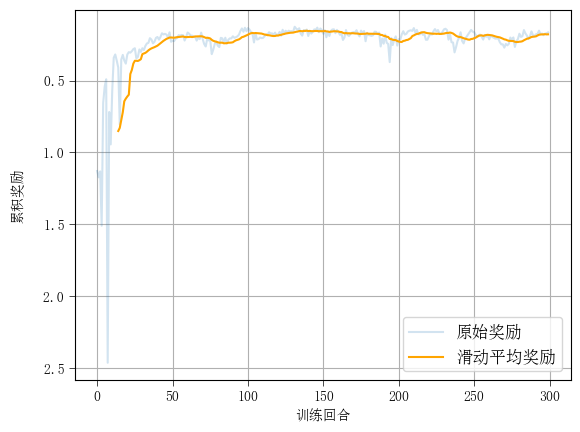
\includegraphics[width=\linewidth]{figures/改进的mappo累积奖励.png}
        \caption{策略网络每个训练回合的累积奖励}
    \end{subfigure}
    \quad
    \begin{subfigure}[t]{0.43\textwidth}
        \centering
        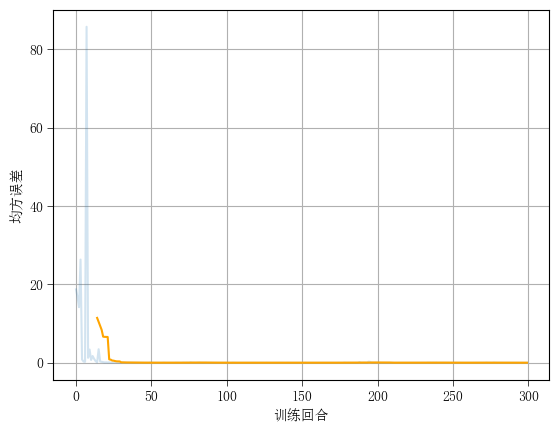
\includegraphics[width=\linewidth]{figures/改进的mappo的均方误差.png}
        \caption{评价网络的均方误差（MSE）}
    \end{subfigure}
    \caption{改进MAPPO模型的训练结果}
    \label{fig:改进的多智能体强化学习模型的训练结果}
\end{figure}

在策略网络的训练结果图中，
蓝色线条表示每个训练回合智能体获得的累积奖励，橙色线条表示为
15个训练回合的滑动平均值。
从图中可以看出，累积奖励曲线在训练初期（前50轮次）呈现显著上升趋势，
表明策略网络（Actor）能够快速学习有效的驻站控制策略，
随着训练轮次的增加（约100轮次后），曲线逐渐趋于平缓，策略网络接近收敛状态，
收敛速度较快，策略优化进入稳定阶段。
由于强化学习算法的探索性和公交系统存在的随机性，累积奖励存在波动。

从图\ref{fig:改进的多智能体强化学习模型的训练结果}（b）评价网络的均方误差
（Mean Squared Error, MSE）可以看出，均方误差（MSE）训练初期快速下降，表明评价
网络（Critic）迅速适应状态价值的动态变化。中后期误差逐步趋近于低值区间，说明价值估计
逐渐精确，可以为策略网络提供可靠的梯度更新方向。同时可以看出，在累积奖励上升阶段
（0-50轮次），均方误差（MSE）同步下降，验证了演员-评论员（Actor-Critic）算法框架的协同优化机制。


\subsection{实验结果与性能分析}
 
为评估训练模型的可靠性，本研究针对每个控制模型展开20回合独立仿真实验。
图\ref{fig:无控制的车辆运行轨迹}呈现了单线环形线路公交系统运行8小时，基于无控制模型（NH），系统中车辆运行的时空轨迹。
该模型中公交车辆运行未施加任何驻站控制干预，从图中可以看出，在缺乏协同控制策略的情况下，
公交车辆因动态扰动传播发生显著串车现象。


% 模型训练结束后，对该模型进行测试验证。每个对比模型通过20回合的模拟来评估其可靠性。
% 首先从微观层面进行分析，下图\ref{fig:无控制的车辆运行轨迹}是无控制模型（NH）的公交车辆运行轨迹图，即在系统中不对公交车辆
% 进行任何驻站控制干预。从图中可以看出，在不采取任何干预措施的情况下，系统中的公交车辆
% 很容易发生串车。


\begin{figure}[!ht]
    \centering
    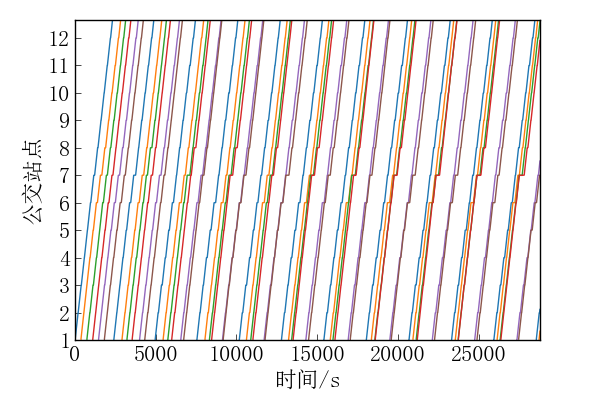
\includegraphics[width=0.62\linewidth]{figures/NH车辆轨迹.png}
    \caption{无控制的车辆运行轨迹}
    \label{fig:无控制的车辆运行轨迹}
\end{figure}
\captionsetup{justification=centering} 
\begin{figure}[!ht] 
    \centering
    \begin{subfigure}[b]{0.47\textwidth}
        \centering
        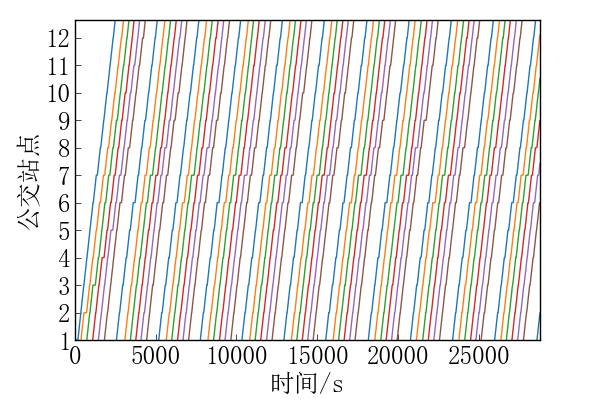
\includegraphics[width=\linewidth]{figures/HH车辆轨迹.png}
        \caption{基于固定车头时距的控制策略}
    \end{subfigure}
    \quad
    \begin{subfigure}[b]{0.46\textwidth}
        \centering
        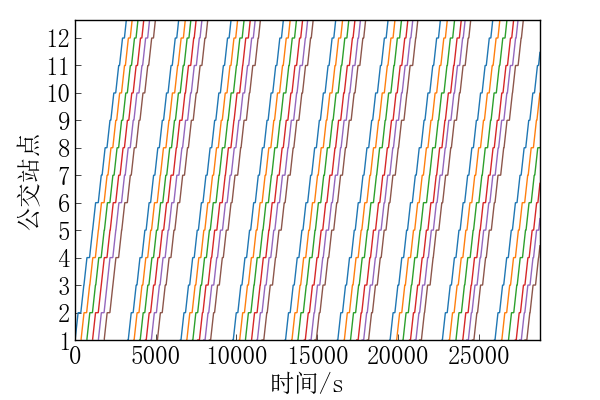
\includegraphics[width=\linewidth]{figures/SH车辆轨迹.png}
        \caption{基于时刻表的控制策略}
    \end{subfigure}
    \vskip 10pt % 子图组间垂直间距
    \begin{subfigure}[b]{0.46\textwidth}
        \centering
        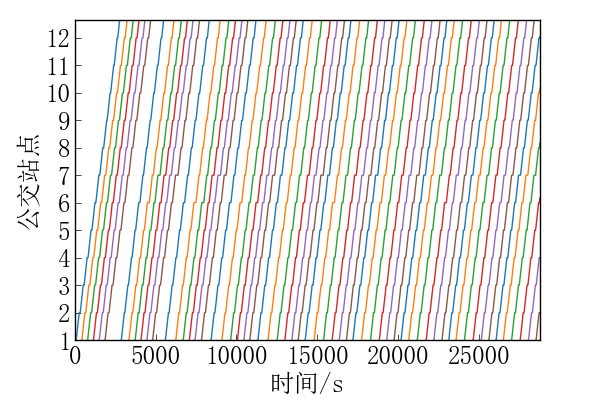
\includegraphics[width=\linewidth]{figures/FH车辆轨迹.png}
        \caption{基于前向车头时距的控制策略}
    \end{subfigure}
    \quad
    \begin{subfigure}[b]{0.46\textwidth}
        \centering
        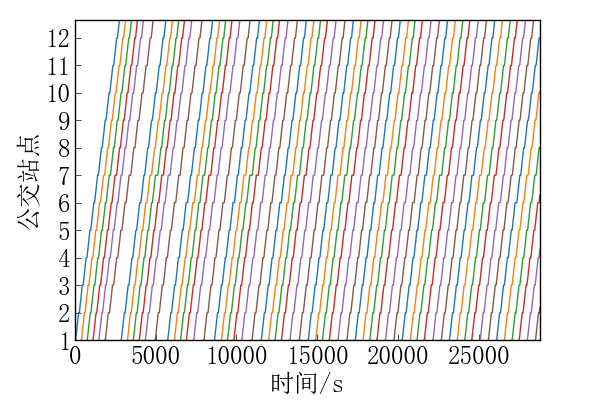
\includegraphics[width=\linewidth]{figures/BH车辆轨迹.png}
        \caption{基于后向车头时距的控制策略}
    \end{subfigure}
    \vskip 10pt % 子图组间垂直间距
    \begin{subfigure}[b]{0.46\textwidth}
        \centering
        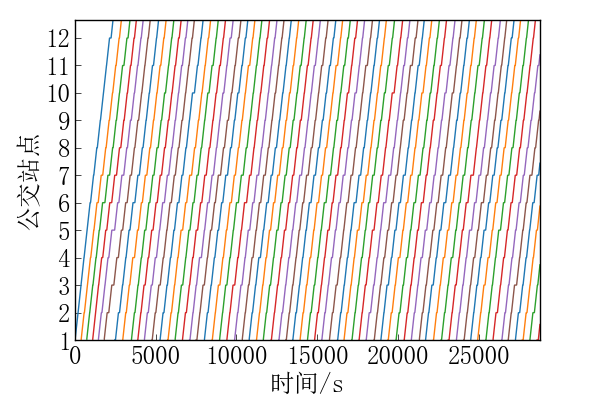
\includegraphics[width=\linewidth]{figures/MAPPO车辆轨迹.png}
        \caption{基于MAPPO算法的控制策略}
    \end{subfigure}
    \quad
    \begin{subfigure}[b]{0.46\textwidth}
        \centering
        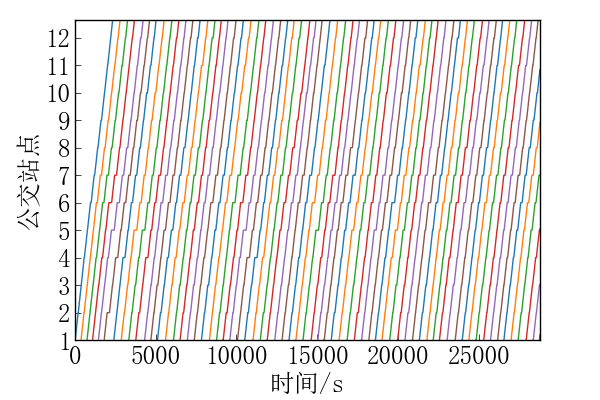
\includegraphics[width=\linewidth]{figures/改进的MAPPO车辆轨迹.png}
        \caption{基于改进MAPPO算法的控制策略}
    \end{subfigure}
    \caption{不同控制策略下的公交运行车辆轨迹}
    \label{fig:不同控制策略下的公交运行车辆轨迹}
\end{figure}

下图\ref{fig:不同控制策略下的公交运行车辆轨迹}是本文所提出的
基于强化学习的控制模型和其他基准模型的车辆轨迹，
基于固定车头时距的控制模型（HH）
和基于时刻表的控制模型（SH）视为是基于规则的控制模型，在一定程度上都可以缓解公交串车的发生，
但对于公交车头时距的不规律问题改善不明显，原因在于，
两种基于规则的控制方法无法灵活有效的处理公交系统出现的不确定性因素，无法有效实现车头时距的规律性。

相比于基于规则的控制，基于前向车头时距（FH）、基于后向车头时距
（BH）以及基于强化学习的控制模型（MAPPO算法和改进MAPPO算法）的控制策略更具灵活性，
从车辆轨迹可以看出，这些策略对于缓解公交串车现象更有效。
相比之下，基于强化学习的控制策略表现更优，
主要是强化学习中智能体可以获取更多的实时信息，
如观测状态中包含了车头时距等信息，使得智能体的决策更优，减少不必要的干预，
而其他控制策略则不能充分利用这一信息，
同时基于强化学习的策略还可以考虑决策的长期影响，在改善公交的车头时距偏差的方面
表现更佳。
\captionsetup{justification=centering}
\begin{figure}[htbp]  
    \centering
    \begin{subfigure}[b]{0.44\textwidth}
        \centering
        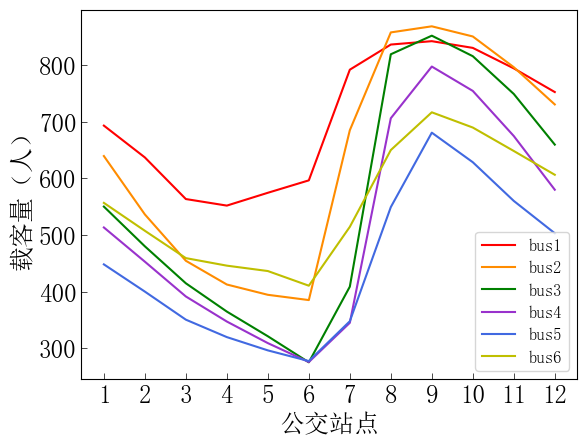
\includegraphics[width=\linewidth]{figures/NH载客量.png}
        \caption{NH策略的公交载客量}
    \end{subfigure}
    \quad
    \begin{subfigure}[b]{0.44\textwidth}
        \centering
        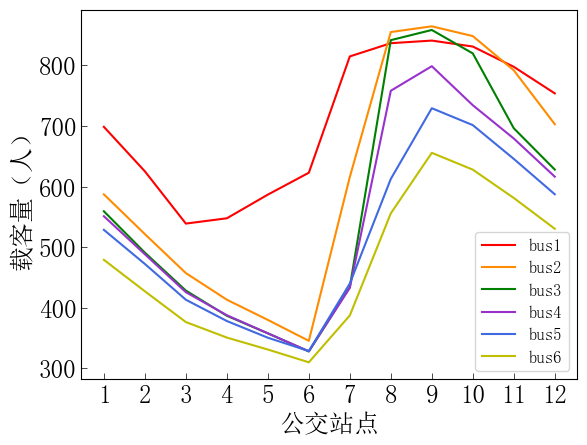
\includegraphics[width=\linewidth]{figures/HH载客量.png}
        \caption{HH策略的公交载客量}
    \end{subfigure}
    \vskip 10pt % 子图组间垂直间距
    \begin{subfigure}[b]{0.44\textwidth}
        \centering
        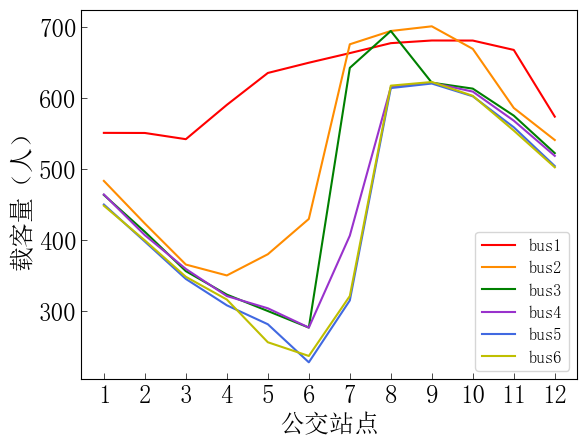
\includegraphics[width=\linewidth]{figures/SH载客量.png}
        \caption{SH策略的公交载客量}
    \end{subfigure}
    \quad
    \begin{subfigure}[b]{0.44\textwidth}
        \centering
        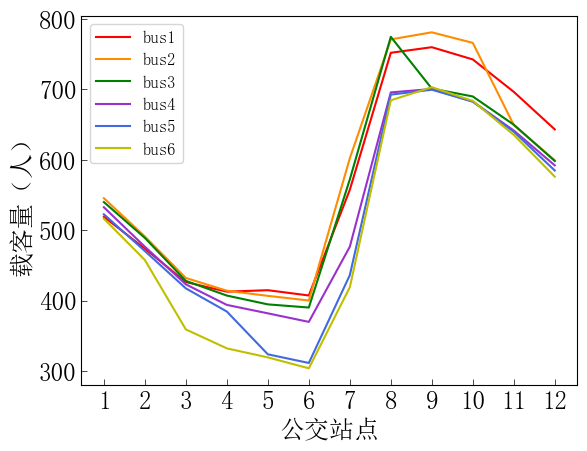
\includegraphics[width=\linewidth]{figures/FH载客量.png}
        \caption{FH策略的公交载客量}
    \end{subfigure}
    \vskip 10pt % 子图组间垂直间距
    \begin{subfigure}[b]{0.44\textwidth}
        \centering
        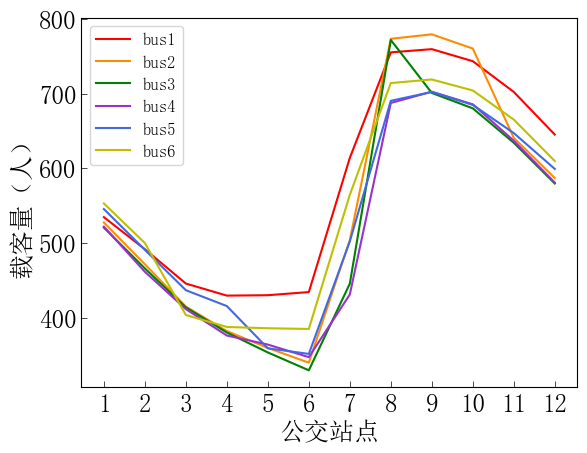
\includegraphics[width=\linewidth]{figures/BH载客量.png}
        \caption{BH策略的公交载客量}
    \end{subfigure}
    \quad
    \begin{subfigure}[b]{0.44\textwidth}
        \centering
        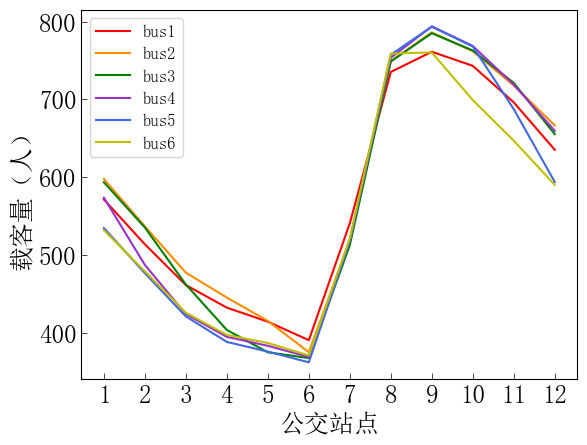
\includegraphics[width=\linewidth]{figures/MAPPO载客量.png}
        \caption{基于MAPPO算法策略的公交载客量}
    \end{subfigure}
    \vskip 10pt % 子图组间垂直间距
    \begin{subfigure}[t]{0.44\textwidth}
        \centering
        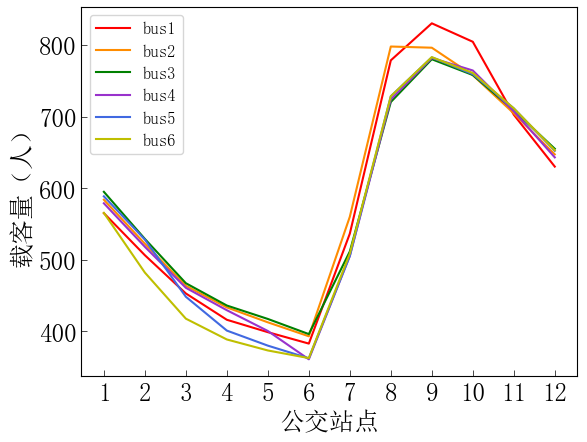
\includegraphics[width=\linewidth]{figures/改进的MAPPO载客量.png}
        \caption{基于改进MAPPO算法策略的公交载客量}
    \end{subfigure}
    \caption{不同策略下不同公交站点各车辆的载客量}
    \label{fig:不同策略下不同公交站点各车辆的载客量}
\end{figure}

图\ref{fig:不同策略下不同公交站点各车辆的载客量}是整个模拟过程中，
不同的控制策略下，系统中公交车辆在每个站点的累积载客数量，
每个子图中的不同线条表示不同的车辆。从图中可以看出，在没有任何控制干预（NH）的情况下，
系统中车辆的载客辆高度不均，存在资源浪费，
同时从乘客的角度来看，存在部分车辆过度拥挤导致乘客出行体验不佳。
基于固定车头时距的控制策略（HH）和基于时刻表的控制策略（SH）对于车辆载客量的均衡
改善较小，相比之下，
基于前向车头时距的控制策略（FH）和基于前向车头时距的控制策略（BH）有了一定程度的改善，
因为他们可以较好的缓解公交串车的发生。
同样的，基于强化学习的控制策略表现更优，对比两种强化学习方法，
从图\ref{fig:不同策略下不同公交站点各车辆的载客量}（f）和（e）可以看出，
本文所提出的基于改进的MAPPO算法的控制策略在均衡车
辆载客量方面表现最佳，更有效缓解的了公交串车和载客量不均衡的问题。


% \captionsetup{justification=centering} % 设置题注内容居中
% \begin{figure}[!ht]
%     \begin{minipage}[t]{0.5\linewidth}
%         \centering
%         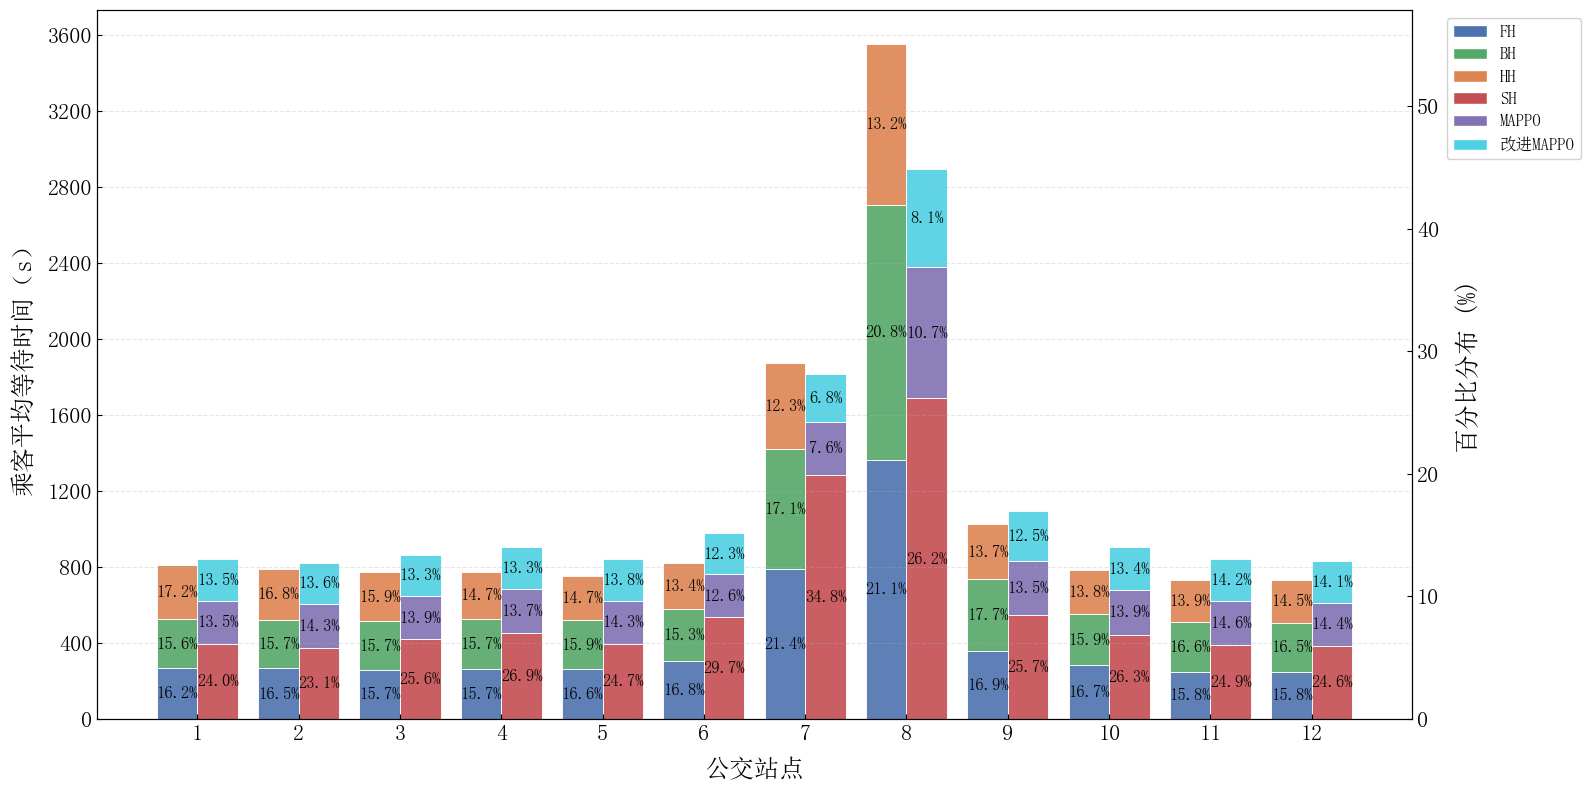
\includegraphics[width=\textwidth]{figures/AWT.png}
%         \caption{不同策略下的乘客平均等待时间\\（AWT）}
%         \label{fig:平均等待时间}
%     \end{minipage}%
%     \begin{minipage}[t]{0.5\linewidth}
%         \centering
%         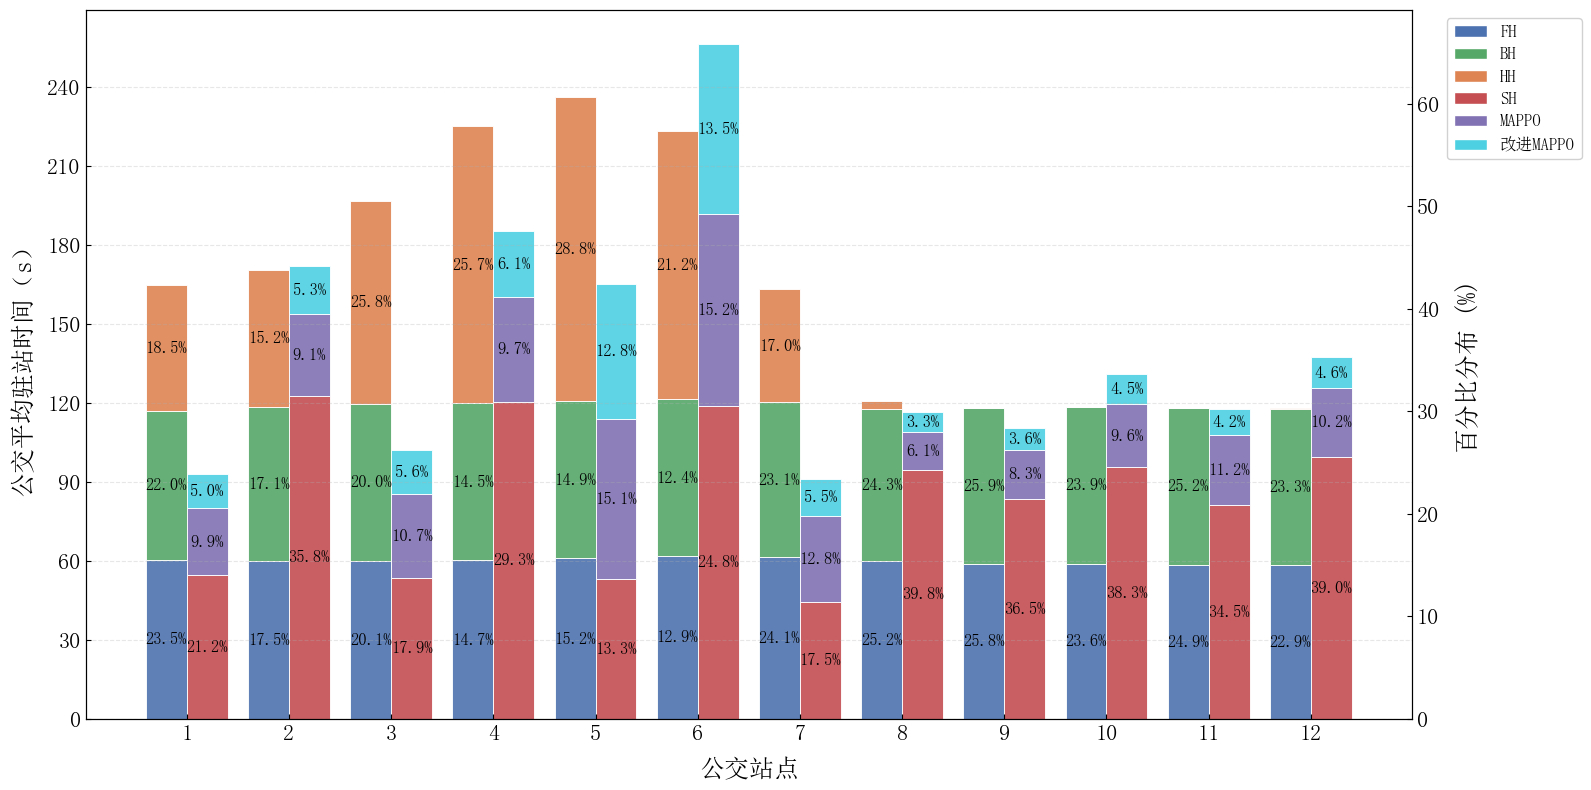
\includegraphics[width=\textwidth]{figures/AHT.png}
%         \caption{不同策略下的车辆平均驻站时间\\（AHT）}
%         \label{fig:平均驻站时间}
%     \end{minipage}
% \end{figure}

% \captionsetup{justification=centering} % 设置题注内容居中
% \begin{figure}[htbp]
%     \begin{minipage}[t]{0.5\linewidth}
%         \centering
%         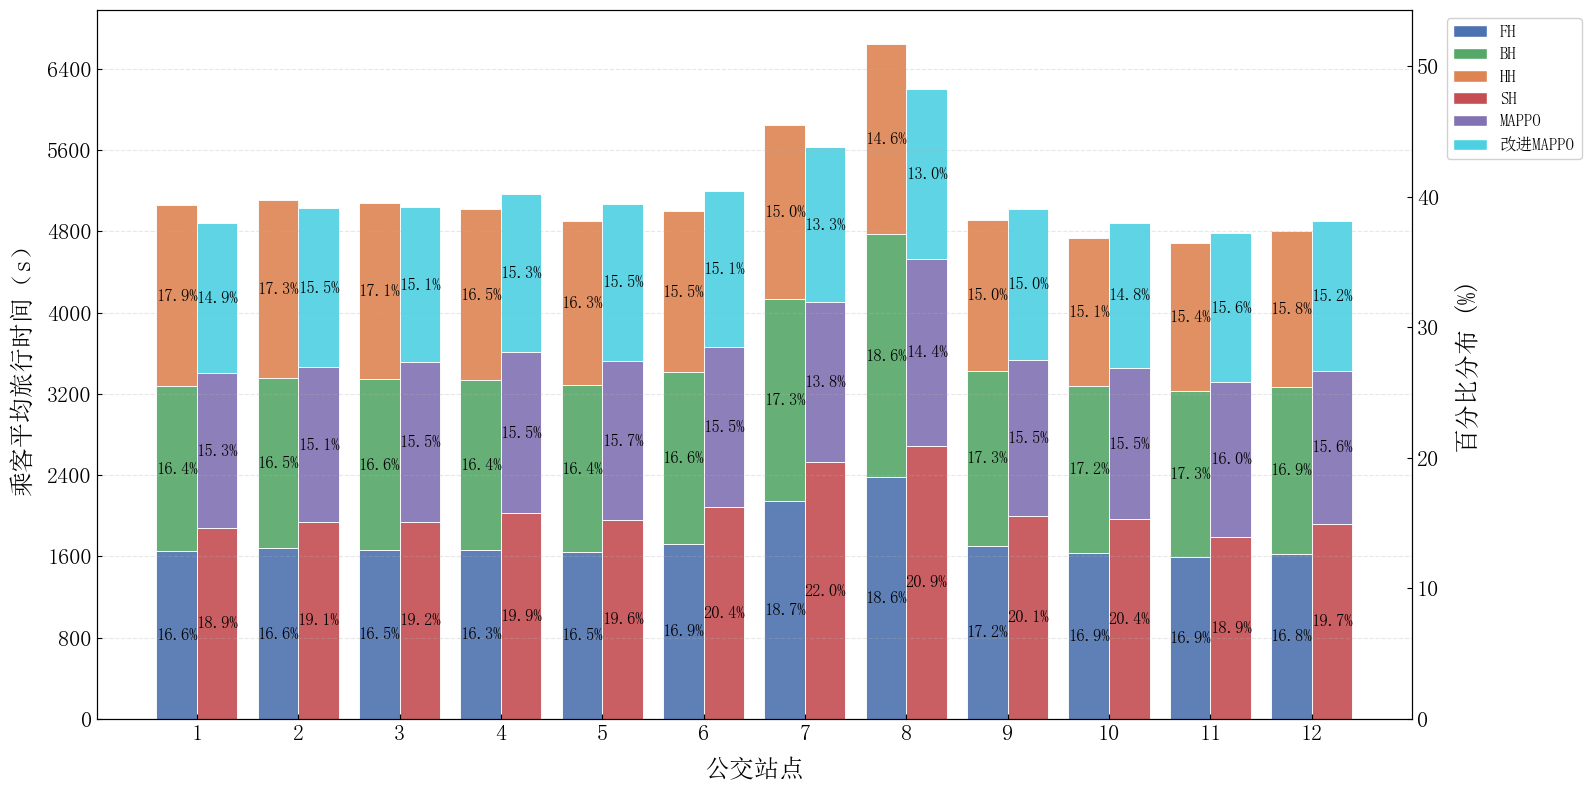
\includegraphics[width=\textwidth]{figures/ATT.png}
%         \caption{不同策略下的乘客平均旅行时间\\（ATT）}
%         \label{fig:平均旅行时间}
%     \end{minipage}%
%     \begin{minipage}[t]{0.5\linewidth}
%         \centering
%         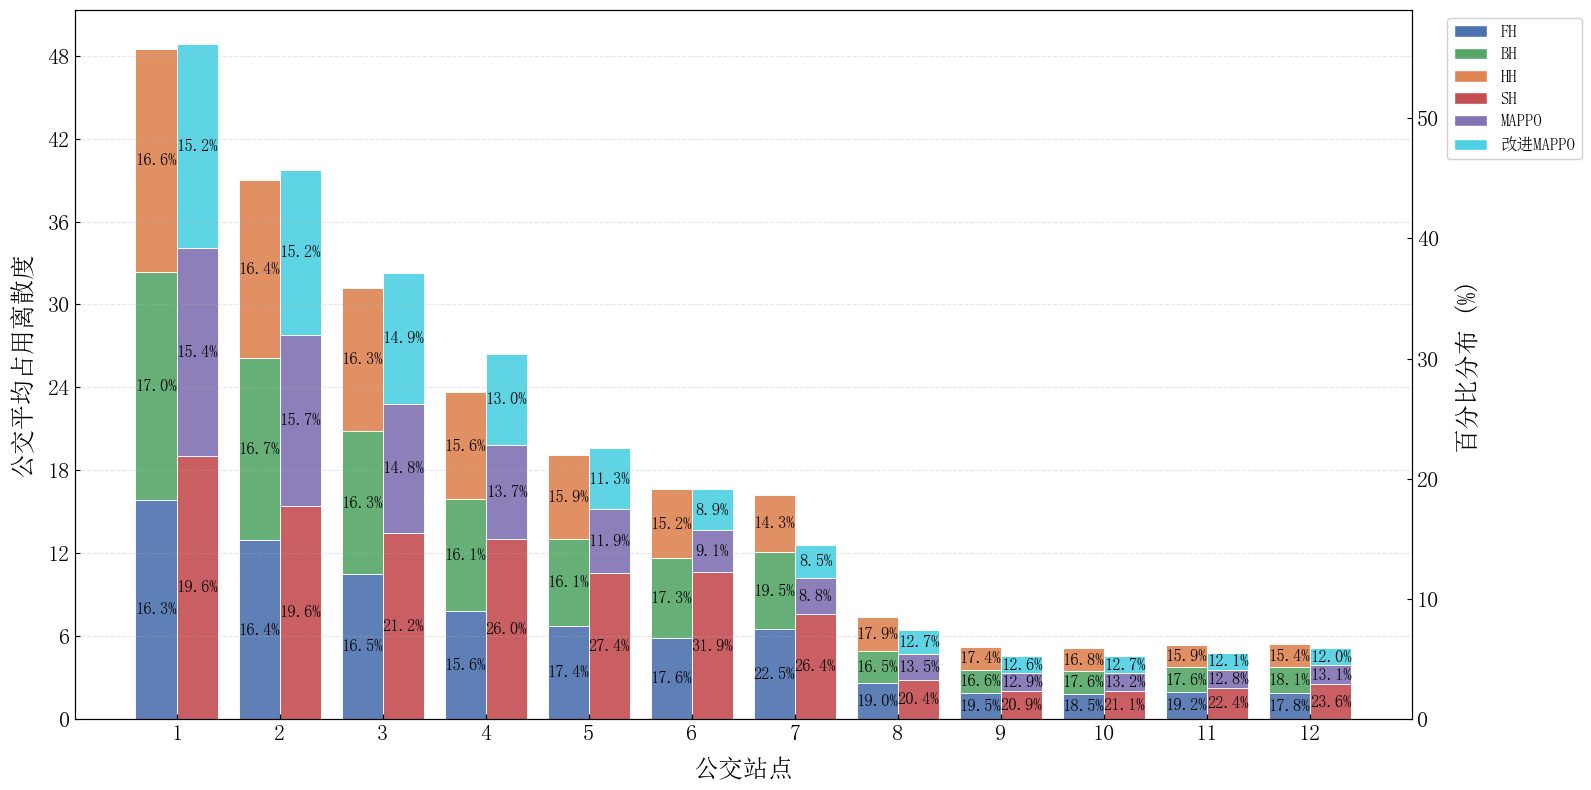
\includegraphics[width=\textwidth]{figures/AOD.png}
%         \caption{不同策略下的车辆平均占用离散度\\（AOD）}
%         \label{fig:平均车辆占用离散度}
%     \end{minipage}
% \end{figure}


为解析控制策略的宏观影响，下图\ref{fig:平均等待时间}至图\ref{fig:平均车辆占用离散度}
分别展示了不同控制策略下站点乘客的平均等待时间（AWT）、车辆平均驻站时间（AHT）、
乘客平均旅行时间（ATT）和车辆平均占用离散度（AOD）的分布特征。

\begin{figure}[!ht]
    \centering
    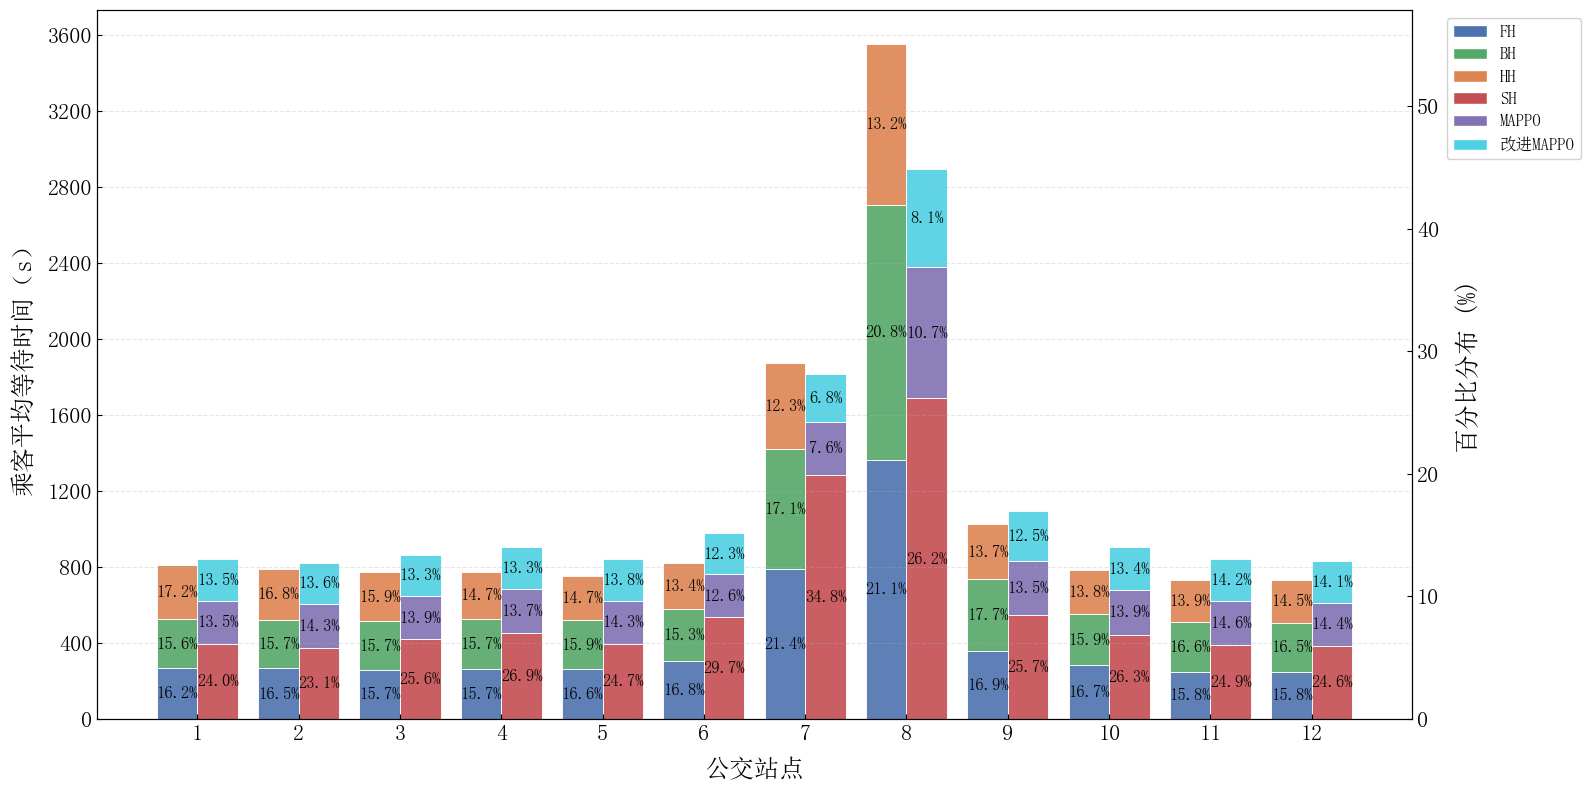
\includegraphics[width=1.\linewidth]{figures/AWT.png}
    \caption{不同策略下的乘客平均等待时间（AWT）}
    \label{fig:平均等待时间}
\end{figure}

图\ref{fig:平均等待时间}为不同控制策略下公交系统各公交站点乘客平均等待时间（AWT）与
对应百分比分布的堆叠柱状图。横轴表示公交站点；左侧纵轴为乘客平均等待时间，右侧纵轴
为各控制策略在对应站点乘客平均等待时间的百分比分布。图中的不同颜色条代表不同控制策略
（如FH、BH等），数据条的长度反映各策略下乘客平均等待时间（AWT）的数值的大小，
百分比通过单个策略AWT值比站点所有策略AWT值总和计算得出。

图\ref{fig:平均等待时间}可以看出，基于强化学习的控制策略（MAPPO算法及改进MAPPO算法）
在AWT指标上显著优于传统基准方法。基于时刻表的控制策略（SH），因动态
适应性不足，其乘客平均等待时间（AWT）比其他策略长得多。尽管两种基于强化学习的控制策略
在该指标上的表现差异较小，但基于改进MAPPO算法的控制策略仍然有更好的表现。

\begin{figure}[!ht]
    \centering
    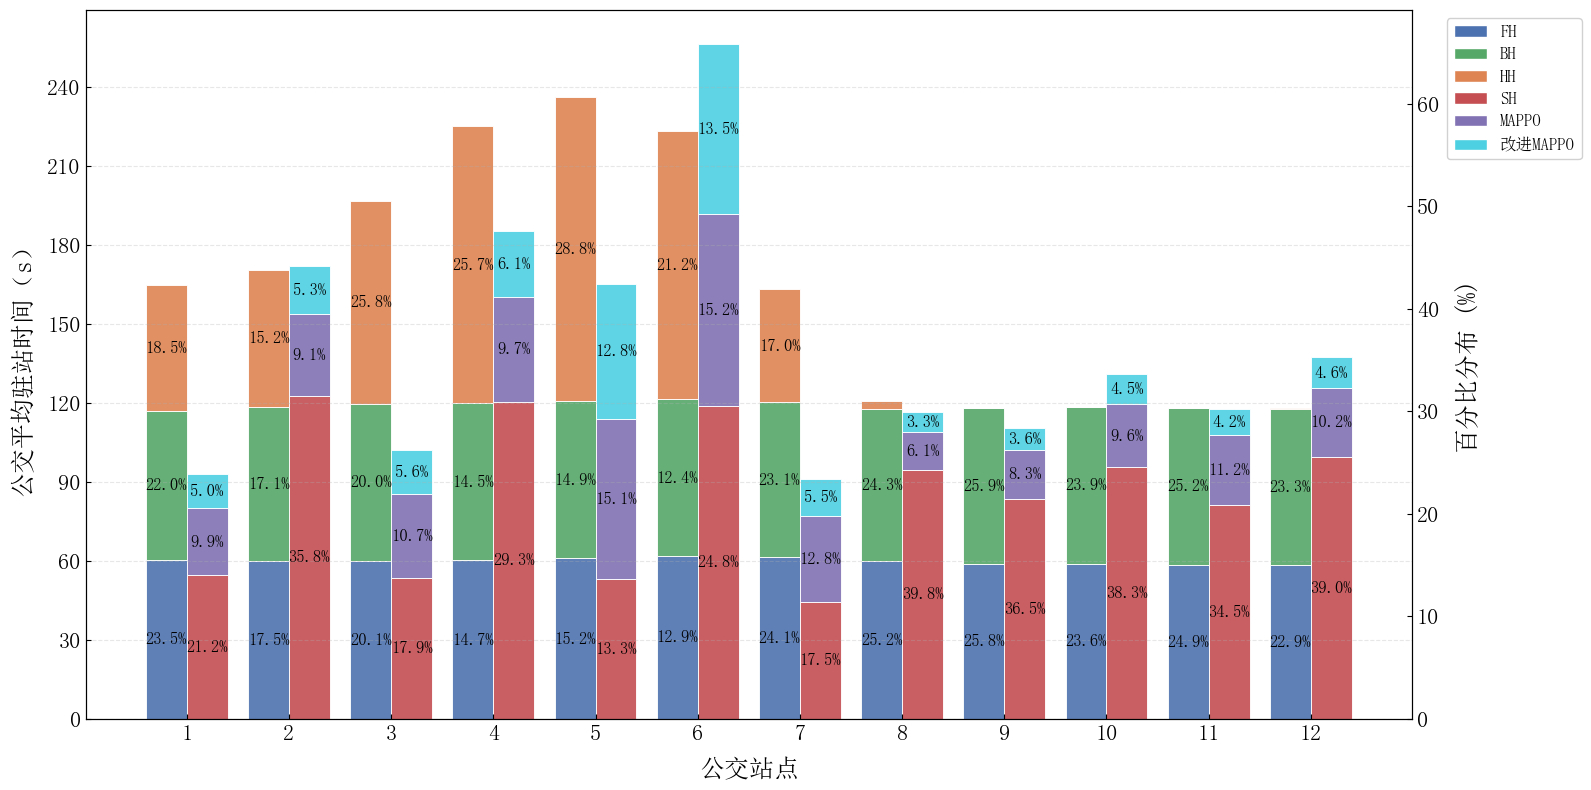
\includegraphics[width=1.\linewidth]{figures/AHT.png}
    \caption{不同策略下的车辆平均驻站时间（AHT）}
    \label{fig:平均驻站时间}
\end{figure}

图\ref{fig:平均驻站时间}呈现了公交系统运行过程中各站点车辆的平均驻站时间（AHT），
可以看出，基于强化学习算法的策略在该指标上优势显著，尤其是基于改进 MAPPO 算法的驻站控制策略，
其平均驻站时间最小。该结果表明，本文提出的模型能够通过较低程度的控制干预，
实现公交系统车头时距均衡，进而有效抑制串车现象。
图中基于固定车头时距的控制策略（HH），在$s_{9}$至$s_{12}$站点未实施控制干预，
而在$s_1$至$s_7$的站点施加了较多的控制干预。推测其原因：该策略在车辆
运行初期通过控制干预维持车头时距的稳定，使得后期部分站点暂时无需驻站控制；
随着系统运行，可能出现车头时距失衡问题，但本节公交系统
模型为环形线路，当车头时距不稳定时，车辆可能循环返回至先前进行过控制干预的站点，
最终呈现出公交在$s_1$到$s_7$站点有了较多的控制干预。

\begin{figure}[!ht]
    \centering
    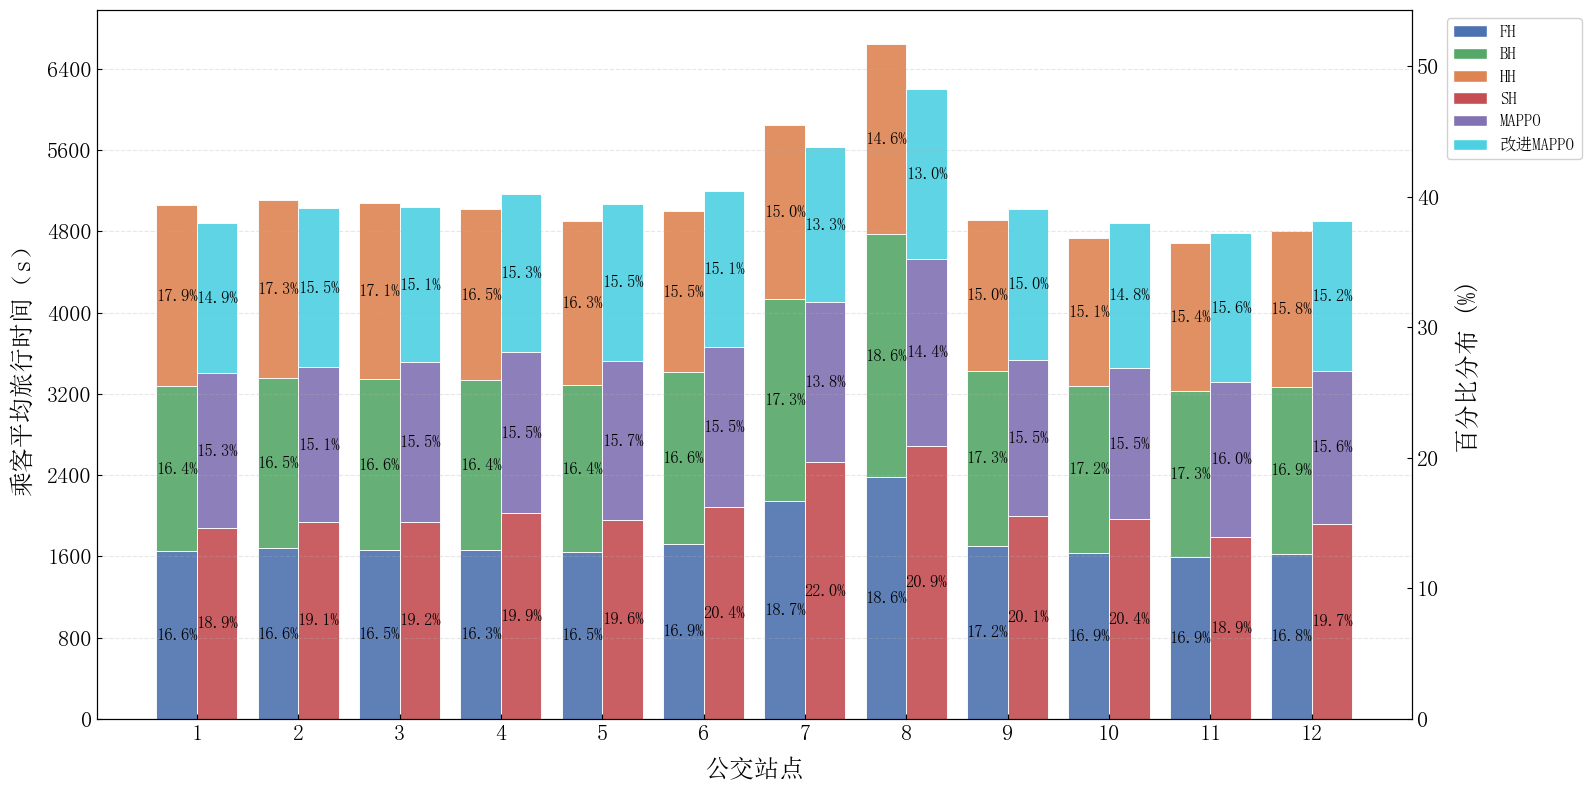
\includegraphics[width=1.\linewidth]{figures/ATT.png}
    \caption{不同策略下的乘客平均旅行时间（ATT）}
    \label{fig:平均旅行时间}
\end{figure}

图\ref{fig:平均旅行时间}是公交系统运行过程中，在各站点乘客的平均旅行时间
（定义为乘客自进入公交系统等待上车起至完成行程的全程耗时）。
图中分析可知，与其他策略相比，基于强化学习的驻站控制策略在该指标上展现出更优的性能，
而本文提出的控制策略（改进MAPPO算法）在该指标上表现最佳，乘客的平均旅行时间最短。

\begin{figure}[!ht]
    \centering
    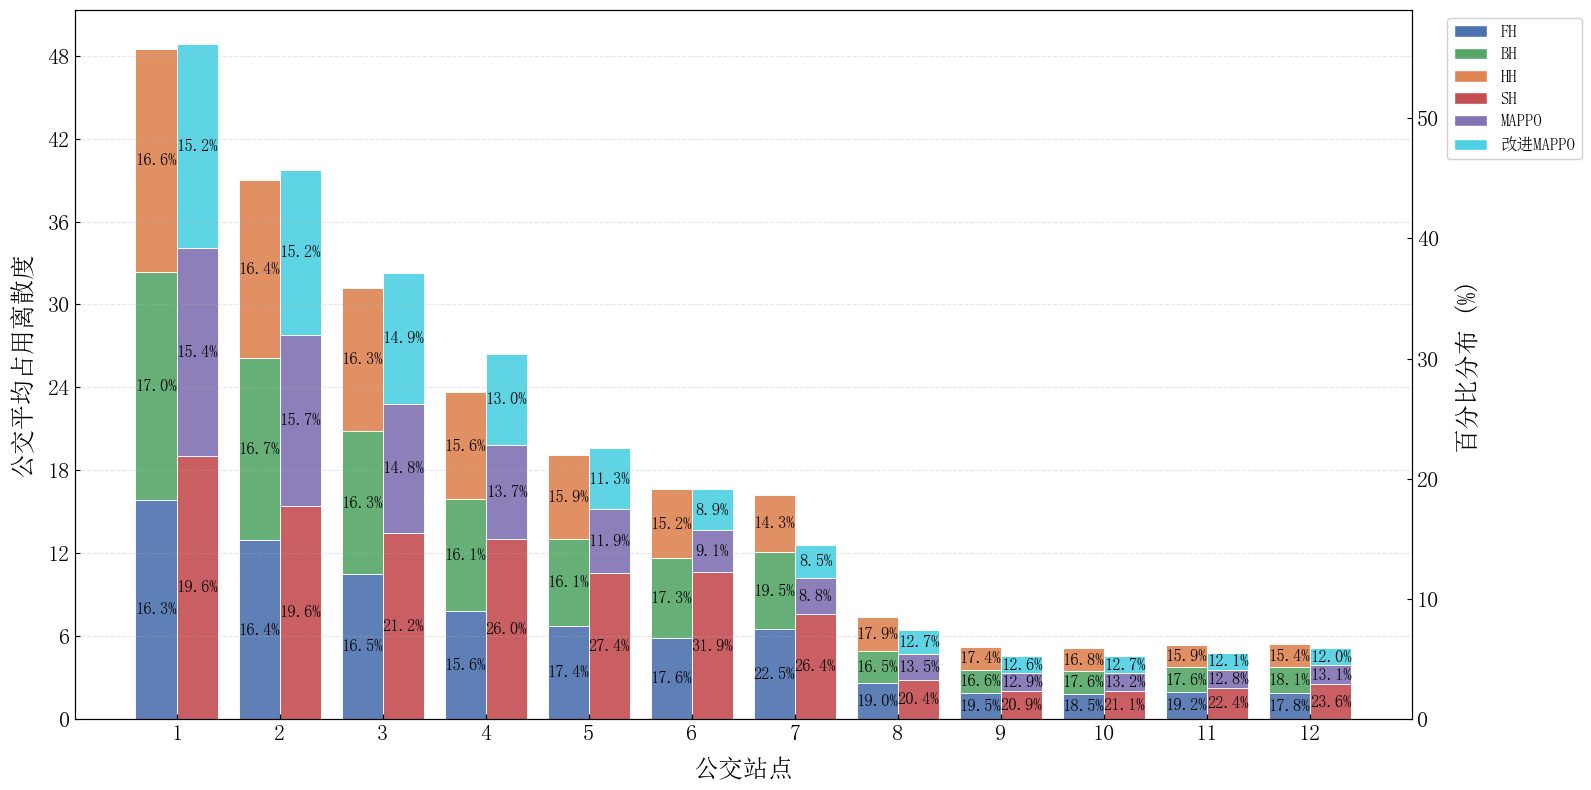
\includegraphics[width=1.\linewidth]{figures/AOD.png}
    \caption{不同策略下的车辆平均占用离散度（AOD）}
    \label{fig:平均车辆占用离散度}
\end{figure}

图\ref{fig:平均车辆占用离散度}量化了不同控制策略下公交站点的车辆占用离散度（AOD），
该指标通过表征车辆时空资源分布的均衡性，反映系统运行的动态平稳性。实验结果显示，
本文提出的基于改进MAPPO算法的控制模型显著降低了AOD值，再该指标上表现出良好的性能。

% 是公交系统运行过程中每个站点车辆占用的离散度（AOD），通过衡量资源
% 的利用效率侧面反映公交系统的平稳性，图中可以直观的感受本文所提出的控制模型的较好性能。

本节通过多维度评估揭示了不同驻站控制策略的性能差异。结果表明，基于规则的驻站控制策略
（特别基于时刻表的控制策略SH）存在显著的适应性局限，驻站控制干预程度较大，
驻站控制时间更长，乘客的出行时间成本更大，这验证了动态控制策略在提升公交运营效率
方面的必要性。本文提出的改进MAPPO算法展现出显著的系统优化能力，
在四个指标中表现最佳且更稳定。表明了智能体之间的协调控制和长期奖励对于控制策略的
稳定性和可靠性至关重要。
总体来看，基于改进MAPPO算法的控制策略可以在引入较少的干预的情况下，有效缓解公交串车问题，
保持车头时距的稳定，
减少乘客的等待时间和均衡车辆的载客量，提供更优的服务。

% 从整个过程来看，基于规则的驻站控制策略，尤其是基于时刻表的驻站控制策略（SH）不够灵活，
% 干预程度更大，驻站控制时间更长，而且
% 因其性能不佳，相比于其他策略，乘客的时间成本更大，
% 这验证了适当的驻站控制可以有效提升公交系统的运行效率。
% 本文所提出的策略在仿真模拟过程中可以有效防止串车的发生，因此
% 同时也表明了，



\section{实例分析}
% \section{问题描述}
在上一节的研究中，研究场景设定为理想化环形公交线路，其核心假设包括：
（1） 采用闭环运行机制，车辆沿固定路径进行无限循环行驶；（2）运行周期通过预设时间
阈值控制，当累计运行时长达到设定值时系统自动终止；（3）站点空间分布遵循均匀离散化原
则，站间距保持恒定；（4）车辆运行动力学模型采用匀速运动假设，忽略实际交通环境中的速
度波动因素。该简化模型为算法验证提供了可控实验环境，但其简化条件与实际公交运营场景存在显著差异。
具体表现为：
实际道路环境中，车辆行驶速度受交通信号、突发拥堵及驾驶
行为等动态扰动因素影响呈现显著随机性特征；公交站点通常依据客流需求
进行非均匀优化布局，导致站间距通常不是等距的；
公交线路普遍采用起讫点式拓扑结构，而非无限循环运行模式。
为提升算法工程适用性，本节将提出的强化学习模型应用于更现实的场景，
提出一种广义公交运行仿真框架，考虑公交运行中各种干扰因素对公交运行速度的时变影响
、真实公交发车间隔及非均匀公交站点分布等多种现实因素。

% \subsection{研究假设与简化条件}
% 在公交驻站控制建模中，实际运行场景的复杂性需通过合理的假设进行抽象化处理，
% 以聚焦核心控制逻辑的构建。本研究基于前人研究文献中的一些常见假设，结合
% 公交驻站控制问题的特性，提出以下假设：

% （1）\textbf{车辆同质性假设}：
% 线路上所有公交车辆的性能参数（如动力特性、能耗效率）
% 及运营成本（如单位时间维护费用）均保持同质化。

% （2）\textbf{载客容量均一性假设}：
% 所有车辆的最大载客容量恒定，该假设旨在避免因为车辆容量差为模型带来复杂性，
% 使研究更专注与乘客需求和车辆供给之间的匹配。

% （3）\textbf{乘客候车行为确定性假设}：
% 乘客候车耐心服从理想化分布，即所有到站乘客均会等待至车辆到达，不存在因等待
% 时间超出心理阈值而放弃乘车的流失行为。此假设简化了乘客流失对运营效果的影响，
% 使研究聚焦于驻站控制策略本身的性能验证。

\subsection{线形公交系统建模框架}
\label{sec:linear_model}
\begin{figure}[!ht]
    \centering
    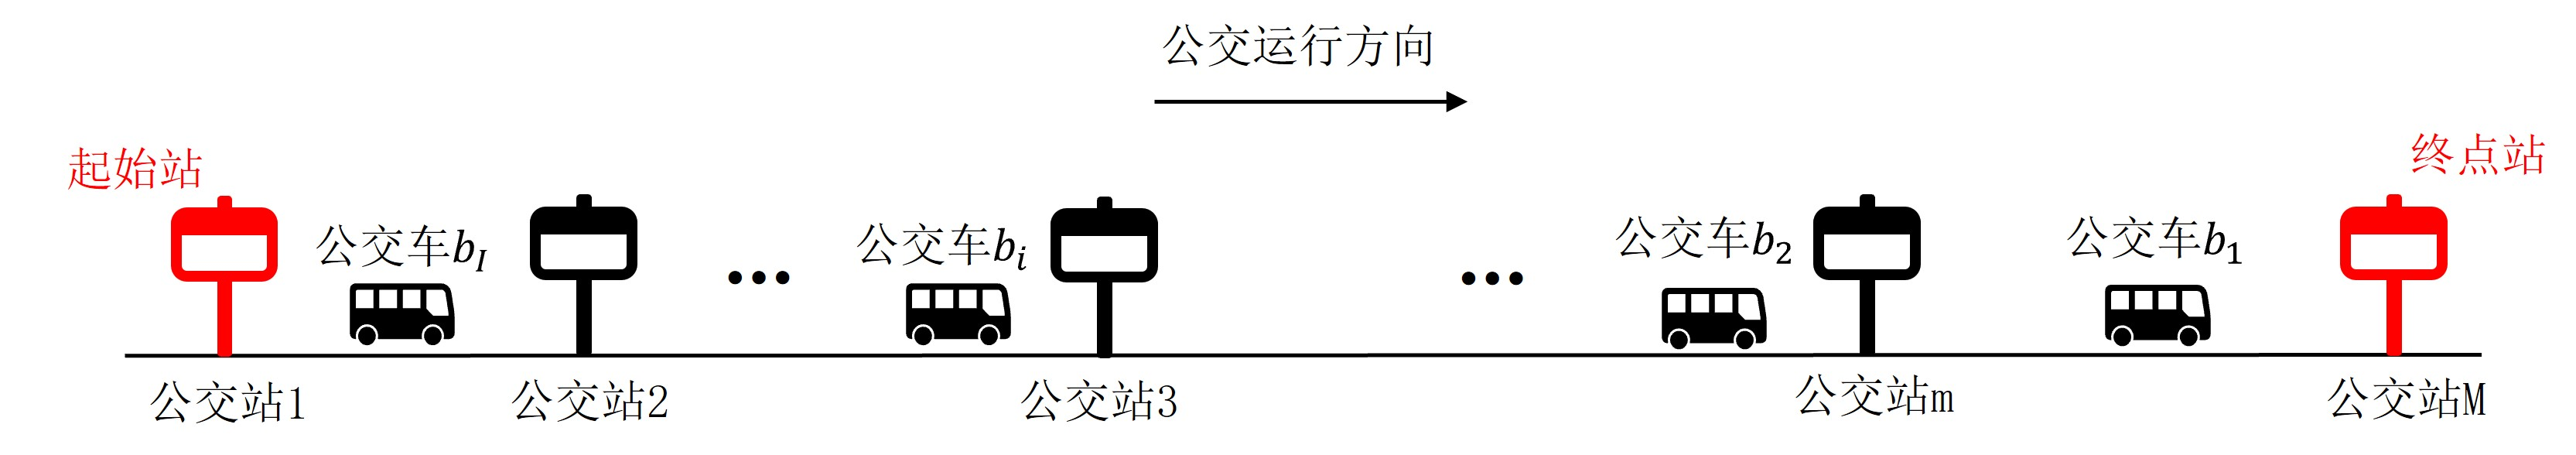
\includegraphics[width=0.99\linewidth]{figures/线性线路公交运行图.jpg}
    \caption{线形公交线路运行图}
    \label{fig:公交运线路图}
\end{figure}
本节研究针对具有起讫点结构的线形公交线路系统展开建模，线形公交运行线路如上图\ref{fig:公交运线路图}所示，
系统定义如下：

（1）路拓扑与参数设定
\begin{itemize}
    \item 线路总长为$L$，沿线均匀分布$M$个公交站点，记为集合$S = \{s_1, s_2, \ldots, s_M\}$，
    其中$s_1$为起始站点，$s_M$为终点站点；
    \item 运营车队规模为$N$，车辆集合$\mathcal{B}  = \{b_1, b_2, \ldots, b_N\}$，
    所有车辆按发车时刻表$\mathcal{T} = \{t_1, t_2, \ldots, t_N\}$从$s_1$依次投入运营。
\end{itemize}

（2）车辆运行逻辑

车辆$b_i$的运行过程遵循以下规则：
\begin{itemize}
    \item 站点服务：车辆到达站点$s_j$时，停站执行乘客上下车操作：
    \item 驻站决策：站点服务完成后，基于实时状态，车辆决策是否触发驻站控制。
    若进行驻站，则等待相应驻站时长后离站；否则立即驶离。
    \item 终止条件：车辆抵达$s_M$后，在车乘客全部下车，车辆离开公交线路，
    完成单程服务
\end{itemize}



% \subsection{公交线形线路运行模型}
% 本节研究针对具有起讫点结构的线性公交线路系统展开，线形公交运行线路如下图\ref{fig:公交运线路图}所示，
% 系统定义如下：

% （1）线路拓扑与参数设定

% 本章考虑一条长为$L$的线形公交线路系统，线路上包含N辆公交车和M个公交站点。线路上的公交从
% 起始站点按发车时刻表顺序发车，沿着公交线路依次为下游站点提供服务。
% 当车辆抵达某一站点时，停站等待乘客上下车，然后决策是否进行驻站，若不进行驻站，
% 车辆直接驶离该站点，继续前往下一个站点，若车辆进行驻站控制，需要等待驻站
% 时间结束后离开该站点驶向下一站点，如此循环至车辆抵达终点站，在终点站等待车上全部乘客下车后，
% 公交即完成服务，离开线路，。

\subsection{研究假设与系统约束}
在公交驻站控制建模中，实际运行场景的复杂性需通过合理的假设进行抽象化处理，
以聚焦核心控制逻辑的构建。本研究基于前人研究文献中的一些常见假设，结合
公交驻站控制问题的特性，提出以下假设：

（1）车辆同质性假设：
线路上所有公交车辆的性能参数（如动力特性、能耗效率）
及运营成本（如单位时间维护费用）均保持同质化。

（2）载客容量均一性假设：
所有车辆的最大载客容量恒定，该假设旨在避免因为车辆容量差异为模型带来复杂性，
使研究更专注与乘客需求和车辆供给之间的匹配。

（3）乘客候车行为确定性假设：
乘客候车耐心服从理想化分布，即所有到站乘客均会等待至车辆到达，不存在因等待
时间超出心理阈值而放弃乘车的流失行为。此假设简化了乘客流失对运营效果的影响，
使研究聚焦于驻站控制策略本身的性能验证。

基于上述线形公交线路的拓扑结构与研究假设，本节定义系统运行的数学约束条件与
动态交互规则。符号定义与表\ref{tab3-1}一致。

（1）顺序约束

车辆按照系统发车时刻表从起始站点$s_1$顺序发出，并严格遵循非超车原则，车辆$b_{i}$
发车时间晚于车辆$b_{i-1}$，如下式（\ref{顺序约束}）所示。其中$t_{i}^{\mathrm{depart}}$
表示公交车辆$b_{i}$的发车时刻，该约束保证车辆$b_{i}$始终位于$b_{i-1}$上游，形成稳定跟随队列。
% 因此在整个系统运行过程中，车辆$b_{i+1}$始终位于车辆$b_{i}$的上游
% 方向，始终跟随车辆$b_{i}$运行。
\begin{equation}\label{顺序约束}
    t_{i-1}^{\mathrm{depart}} > t_{i}^{\mathrm{depart}} \quad \forall i \in \{1,2,\ldots,N\}.
\end{equation}

（2）车辆到站时间

对于公交线路上的起始站点$s_1$，车辆$b_i$到达该站点的时间即车辆在系统中的发车时刻，由
系统中车辆的发车时刻表决定。车辆$b_i$到达其他站点$s_j$（$j=$2,3,...,$M$）的时间$ta_{i,j}$取决于车辆离开前一站点
$s_{j-1}$（$j=$1,2,...,$M$）的时间$td_{i,j-1}$和在站间运行时间$t_{i,j-1}$，
数学表示式见下式（\ref{到站时间}）。
\begin{equation}\label{到站时间}
    \begin{cases}
    ta_{i,1} \text{取决于发车时刻表} & i= 1,2,...,N\\
    ta_{i,j} = td_{i,j-1} + t_{i,j-1} & i= 1,2,...,N; j = 2,3,...,M.
    \end{cases}
\end{equation}

（3）车辆离站时间

车辆离开当前站点的时间由车辆到达该站点的时间$ta_{i,j}$、等待乘客上下车的时间$\omega_{i,j}$
和车辆在站点的驻站时间$th_{i,j}$三者共同决定，表达式见式（\ref{车辆离开站点的时间}）。

（4）车辆在站点的服务时间

车辆在站点的服务时间$\omega_{i,j}$定义为完成乘客上下车操作所需的时间，服务时间与乘客流量呈线性正相关。
对于起始站点$s_1$，由于仅存在乘客上车行为，其服务时间由单人上车平均耗时$t_b$（单位：秒/人）
和本站实际上车乘客数$\hat{u}_{i,1}$决定；在终点站$s_{M}$，由于只存在乘客下车行为，
停留服务时间由所有乘客的下车总用时决定，取决于下车乘客数量$A_{i,M} $和单人下车平均耗时$t_{a}$（单位：秒/人）；
在中间站点，车辆的服务时间由该站点所有乘客上车、下车总用时中的最大值决定，数学表达式如下
式（\ref{服务时间}）所示。

\begin{equation}\label{服务时间}
    \begin{cases}
    \omega_{i,1} = t_{b} \cdot \hat{u}_{i,1} & i= 1,2,...,N\\
    \omega_{i,j} = \max \{ t_{a}A_{i,j} ,t_{b}\hat{u}_{i,j}\}  & i = 1,2,...,N; j = 1,2,...,M\\
    \omega_{i,M} = t_{a} \cdot A_{i,M} & i= 1,2,...,N.
    \end{cases}
\end{equation}

% 其中$A_{i,M} $ 为在终点站下车的乘客数量。

% 见下式（\ref{车辆在起始点的服务时间}）所示。
% \begin{equation}\label{车辆在起始点的服务时间}
%     \omega_{i,1} = t_{b} \cdot \hat{u}_{i,1}
% \end{equation}
% 在终点站$s_{M}$只有乘客下车过程，停留服务时间由所有乘客的下车总用时决定，见下式（\ref{车辆在终点站的服务时间}）所示，
% 其中$A_{i,M} $ 为在终点站下车的乘客数量。
% \begin{equation}\label{车辆在终点站的服务时间}
%     \omega_{i,M} = t_{a} \cdot A_{i,M}
% \end{equation}
% 在中间站点，车辆的停留服务时间取决于该站点所有乘客上车、
% 下车总用时中的最大值，见式（\ref{车辆在站点的服务时间}）。

（5）站点乘客的总需求

在线形公交线路系统中，除终点站$s_M$（只允许乘客下车）外，其余站点$s_j (j=1,2,...,M-1)$
的乘客到达遵循泊松过程，各站点乘客到达率为$\lambda_{j}$。
公交系统开始运行后，各站点的乘客累积时间遵循以下规则：首辆公交到站前，
其累积乘客的时间为$T$;后续运营阶段，站点累积时间由相邻车辆到站时间间隔动态确定。
站点新增乘客需求$ n_{i,j}$是一个随机变量，表达式见下式（\ref{新增乘客需求}）。
\begin{equation}\label{新增乘客需求}
    \begin{cases}
    n_{i,j} \thicksim \mathsf{P} (\lambda_{i,j},T) & \text{公交站点} s_j(j\neq M) \text{第一次有车辆到站时，}\\
    n_{i,j} \thicksim \mathsf{P} (\lambda_{i,j},h_{i,j}) & \text{否则}
    \end{cases}
\end{equation}

站点乘客的总需求除包含前后两辆
公交车到站间隔内累积的新增乘客需求外，还包含上一辆公交车到站后，由于车辆容量限制
未能登上车辆的剩余乘客$l_{i,j}$，见式（\ref{站点乘客总需求}）。

（6）站点上车人数和滞留乘客人数


站点实际可上车人数受车辆物理容量与运营状态的综合制约，具体表现为：
\begin{itemize}
    \item 最大容许上车人数：对于始发站$s_{i,1}$,由车辆额定容量$U$决定；
    终点站$s_{i,M}$不允许乘客上车；其余中间站点由车辆额定容量$U$、车辆到站时
    在车人数$o_{i,j-1}$和本站下车人数$A_{i,j}$共同决定，表达式如下：
    \begin{equation}
        \hat{u}_{i,j}^{\max} = U - o_{i,j-1} + A_{i,j},\hspace{0.5em} i = 1,2,...,N; j =1,2,...,M-1.
    \end{equation}
    \item 实际上车人数：取决于本站候车总需求$u_{i,j}$和最大容许上车人数$\hat{u}_{i,j}^{\max}$
    中的较小值，表达式如下：
    \begin{equation}
        \hat{u}_{i,j} = \min\{ u_{i,j}, \hat{u}_{i,j}^{\max}\} ,\hspace{0.5em} i = 1,2,...,N; j =1,2,...,M-1.
    \end{equation}
    \item 滞留乘客数量：为保证公交驻站控制模型能够基于
    一个相对稳定的乘客行为模式，乘客按照先到先服务（FIFO）的原则依次上车，
    当站点等待上车的乘客数量$u_{i,j}$超过最大容许上车数量$\hat{u}_{i,j}^{\max}$，
    后面到站的部分乘客会被剩余等待下一辆公交的服务，滞留乘客数量见下式
    （\ref{滞留乘客数量}）。
    \begin{equation}\label{滞留乘客数量}
        l_{i,j} = u_{i,j} - \hat{u}_{i,j}^{\max} ,\hspace{0.5em} i = 1,2,...,N; j =1,2,...,M-1.
    \end{equation}
\end{itemize}



% 站点实际能够登上车辆的最大乘客数量由公交车的容量$U$、车辆到站时的在车乘客数量$o_{i,j-1}$、
% 在站点下车的乘客数量$A_{i,j}$决定，即$U-o_{i,j-1}+A_{i,j}$，若等待上车的乘客数量$u_{i,j}$
% 超过了该站点车辆的最大可上车乘客数量，就会有部分乘客被剩余，为保证公交驻站控制模型能够基于
% 一个相对稳定的乘客行为模式，乘客按照先到先服务的原则依次上车，保证乘客上车的有序性。
% 站点实际能够上车的乘客数量和被剩余的乘客数量见式（\ref{站点实际上车乘客数量}）和式（\ref{站点剩余乘客数量}）。

（7）在车乘客数量

公交$b_{i}$到达站点$s_j$的在车乘客数量即为公交离开上一站点的乘客数量$o_{i,j-1}$，
因此公交离开当前站点时的在车乘客数量$o_{i,j}$由到站时的在车乘客数量$o_{i,j-1}$、
下车乘客数量$A_{i,j}$和实际上车乘客数量$\hat{u}_{i,j}$共同决定，见式（\ref{在车乘客数量}）所示。

（8）下车乘客数量

公交在站点$s_j$的下车乘客数量$A_{i,j}$是是一个随机变量，
乘客仅能在上车站点$s_j$之后的下游站点集合$S_j^+ = \{s_{j+1}, s_{j+2}, ..., s_M\}$中
以相同的概率随机选择下车站点。

% \section{模型构建}
% 本章的建模方式与第3章相同，将公交系统运行中，公交在站点的动态驻站控制构建为一个
% 马尔可夫博弈（Markov Game，MG），将线路上每个公交车视为一个智能体，其强化学习的
% 要素表示如下：

% 状态空间：
% $s_{i,t} = (h^-_{i,t},h^+_{i,t},o_{i,j}/Z)$ 

% 动作空间：
% $a_{i,t} \in [0,1] $

% 奖励函数：
% $  r_{i,t} = -\omega_1\times CV^2 -\omega_2 T^w_{i} $

% 状态转移函数：
% $ \widehat{\mathcal{P}}_{i} : \mathcal{S}_{i} \times \widehat{\mathcal{A}}\mapsto \mathcal{S}_{i}$

% 关于模型的详细理论解释见第3章第3.2节。
% \section{实例分析}
\subsection{公交线路概述}
本章采用的公交系统数据来自成都市T34路公交线路，该线路经过的区域主要集中在天府新区核心区域
（途径华阳客运站、华阳中学、天府新区人民医院等站点）和南部区域（新兴小区、新兴客运站等站点），
上行方向为新兴客运站-香沙路方向，公交运营时段为6：00-19：30，
下行方向为香沙路-新兴客运站方向，运营时段为06:30-20:00，公交票价2元。
公交运行线路如下图\Ref{fig:成都市T34路公交运行线路}所示。
\captionsetup{justification=centering} % 设置题注内容居中
\begin{figure}[!ht] 
    \centering
    \begin{subfigure}[t]{0.48\textwidth}
        \centering
        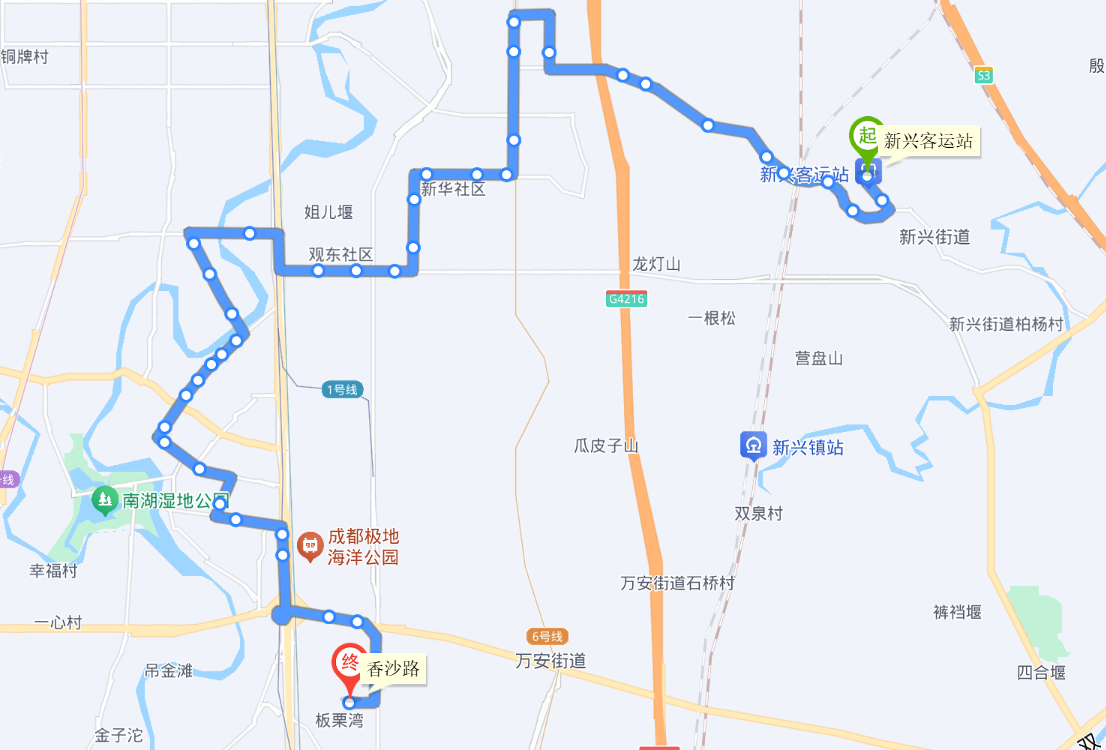
\includegraphics[width=\linewidth]{figures/上行方向.png}
        \caption{上行线路}
    \end{subfigure}
    \quad
    \begin{subfigure}[t]{0.48\textwidth}
        \centering
        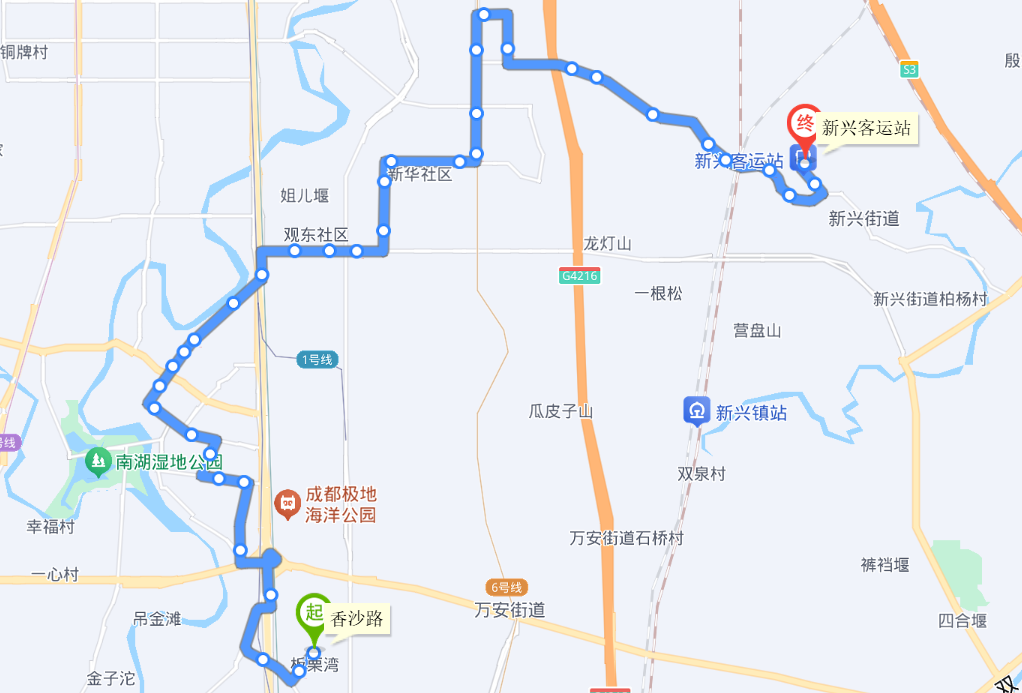
\includegraphics[width=\linewidth]{figures/下行方向.png}
        \caption{下行线路}
    \end{subfigure}
    \caption{成都市T34路公交运行线路}
    \label{fig:成都市T34路公交运行线路}
\end{figure}

\subsection{公交数据处理}
（1）数据准备

本章采用T34路公交上行方向新兴客运站-香沙路方向2022年4月1日的数据公交数据，获取到了该
线路上公交车辆的GPS轨迹数据，包括公交车辆的ID、时间戳、经纬度坐标、速度、方向等信息；
线路公交站点的GPS数据，包含站点的ID、名称、经纬度坐标、所属线路等信息；公交线路信息：
明确线路的起点、终点、途经站点顺序。

（2）GPS轨迹数据预处理

根据车辆ID和线路信息，将数据按线路分组，提取T34路公交上行方向线路数据。
获取的GPS数据中包含可能由于信号遮挡、设备故障等原因产生的无效数据，
使得出现定位精度过低、经纬度值超出合理范围等异常情况，异常数据会干扰后续分析，应
予以剔除。
首先，由于T34路公交线路的运营地理范围在（东经104.055325°-104.098295°，北纬30.477385°-30.548793°），
因此将超出该范围的数据予以剔除。
其次，基于卡尔曼滤波算法（Kalman Filter），利用python中的pykalman库对原始GPS轨迹数据
进行平滑处理，抑制随机噪声与异常波动。
接着设备采集的原始时间戳通过pandas.to\_datetime（）方法转换为标准的日期时间格式
（YYYY-MM-DD  HH:MM:SS），确保时间序列分析的统一基准。
最后采用pyproj库定义坐标参考系，将GPS轨迹数据的经纬度坐标转换至WGS-84地理坐标系。

（3）匹配公交轨迹数据与站点数据

将公交GPS数据与站点GPS数据进行匹配，确定公交是否到达某个站点。
首先进行数据排序，按车辆ID和时间戳对数据进行升序排序，确保数据按时间顺序排列。
根据公交站点的GPS数据，设定匹配阈值为30米，筛选
出车辆轨迹点与各站点之间的距离小于阈值的点，认为公交到达该站点。
采用Haversine公式计算公交车辆轨迹点与站点的距离，计算公式见下式（\ref{Haversine公式}），
\begin{equation}\label{Haversine公式}
    d = 2r \cdot \arcsin\left(\sqrt{\sin^2\left(\frac{\Delta \phi}{2}\right) + \cos(\phi_1) \cdot \cos(\phi_2) \cdot \sin^2\left(\frac{\Delta \lambda}{2}\right)}\right),
\end{equation}
其中$r=6371$ km为地球半径，$\Delta \phi=\phi_2-\phi_1$，$\phi_1$ 、$ \phi_2$ 为两点的纬度
值（以弧度表示），$\Delta \lambda=\lambda_2-\lambda_1$，$\lambda_1$、$\lambda_2$为
两点的经度值（以弧度表示）。  
接着进行时间序列匹配，对匹配成功的轨迹点，记录其到站时间和离站时间。

（4）获取线路公交线路的发车时刻表

根据获取的公交站点的GPS数据和线路数据，确定线路上起点站位置的GPS信息，
采用上述（3）方法找到线路上公交起点站附近的车辆GPS轨迹点。
由于在起点站附近，车辆通常会停留一段时间等待发车，因此，通过计算连续GPS点的时间差来识别
停留时间，如果相邻GPS点的时间差小于一定阈值，则认为车辆仍在停留，过滤停留时间过短或过长的异常
数据，将停留结束后的第一个GPS点的时间戳作为发车时间，将提出取的数据按发车时间和车辆ID进行
排序，形成公交的发车时刻表。

（5）计算公交的站间距离

通过将GPS轨迹点与站点位置进行匹配，提取两个站点之间的所有轨迹点，作为计算站间距离的基础数据。
首先通过Python中的shapely库的LineString类，采用公交的GPS轨迹的经纬度数据进行轨迹线建模，
表示公交的实际行驶路径，然后使用geopandas库的points\_from\_xy函数，分别将获取的车辆GPS轨迹
数据的经纬度信息和公交站点的经纬度信息转换为点几何对象。
合并包含地理几何对象的的公交站点数据和公交实际行驶轨迹线数据，采用Python
计算点在线上的投影距离。具体来说，从线起点开始，沿着线的路径找到对应点垂直
投影到线上的位置，计算从线的起点到这个投影点的距离，这个距离是沿着线的长度来度量的，
而不是两点间的直线距离，最后按照计算出来的投影距离对数据重新排列，
这样就将公交站点的数据插入到了公交的GPS轨迹数据中。
根据公交站点的GPS数据将合并后的数据进行切片操作，计算相邻公交站间的运行距离。

（6）计算公交站间运行速度

根据匹配到的每个公交站点的公交到站、离站时间，可以计算公交相邻站点之间的运行时间
以及公交在站点的停留时间，结合公交站间距离，
计算得到公交在站间的运行速度，剔除异常低速或超速的数据，
根据此来计算全线路平均运行速度和速度方差。
\subsection{实例数据描述}
经过数据处理后，得到的公交数据情况见下表，成都市T34路公交的上行方向：新兴客运站-香沙路方向，
线路全长21 km，包含39个公交站点，两相邻公交站点的站间距如下表\ref{tab4-1}所示。
\begin{table}[!ht]
\centering
\caption{T34路公交站间距离}
\label{tab4-1}
\begin{tabular}{ccccccccccccc}
\toprule
\textbf{编号} & 1-2 & 2-3 & 3-4  & 4-5 & 5-6  & 6-7 & 7-8 & 8-9 & 9-10 \\
\midrule
\textbf{站间距离（m）} & 340 & 590 & 501 & 849 & 861 & 897  & 295 & 600 & 424\\
\toprule
\textbf{编号} & 10-11 & 11-12  & 12-13  & 13-14  & 14-15 & 15-16  & 16-17 & 17-18 & 18-19 & \\
\midrule
\textbf{站间距离（m）}  & 1139 & 439 & 367  & 595 & 377 & 614 & 470 & 422 & 391 \\
\toprule
\textbf{编号} & 19-20 & 20-21 & 21-22 & 22-23  & 23-24 & 24-15& 25-26 & 26-27 & 27-28 \\  
\midrule
\textbf{站间距离（m）} & 697 & 652 & 789 & 407 & 547 & 626 & 266 & 256 & 270  \\
\toprule
\textbf{编号} & 28-29 & 29-30 & 30-31 & 31-32 & 32-33  & 33-34 & 34-35 & 35-36 & 36-37  \\  
\midrule
\textbf{站间距离（m）}& 306 & 372 & 522 & 741 & 369 & 642 & 300 & 1519 & 355 \\
\toprule
\textbf{编号}  & 37-38  & 38-39\\  
\midrule
\textbf{站间距离（m）}& 543 & 673 \\
\bottomrule
\end{tabular}
\end{table}

选取8:15:00-10:40:00作为研究时段，该时段上共运行24辆公交车，线路上公交的发车时刻表
如下表\ref{tab4-2}所示。
\begin{table}[!ht]
\centering
\caption{T34路公交发车时刻表}
\label{tab4-2}
\begin{tabular}{ccccccc}
\toprule
\textbf{公交车辆编号} & 1 & 2 & 3  & 4 & 5  & 6  \\
\midrule
\textbf{发生时刻} & 8:16:03 & 8:22:15 & 8:27:55 & 8:33:47 & 8:40:00 & 8:46:02 \\
\toprule
\textbf{公交车辆编号} & 7 & 8 & 9  & 10 & 11  & 12\\
\midrule
\textbf{发生时刻} & 8:51:41 & 8:58:05 & 9:04:20 & 9:10:15 & 9:16:20 & 9:21:59 \\
\toprule
\textbf{公交车辆编号} & 13 & 14 & 15  & 16 & 17  & 18  \\
\midrule
\textbf{发生时刻} & 9:28:08 & 9:34:10 & 9:39:42 & 9:46:08 & 9:51:44  & 9:57:49 \\
\toprule
\textbf{公交车辆编号} & 19 & 20 & 21  & 22  & 23 & 24 \\  
\midrule
\textbf{发生时刻} & 10:04:04 & 10:10:10 & 10:16:18 & 10:21:45 & 10:27:12 & 10:33:28\\
\bottomrule
\end{tabular}
\end{table}

在该线路上，公交在站间的平均运行速度为25km/h，速度的方差为8.33km/h，
因此为了模拟道路状况的不确定性，
本章将公交在每两个连续车站之间行驶时的速度设置为，$v \times \mathcal{U}(0.8,1.2)$km/h，
其中$v=25$km/h，$\mathcal{U}$表示连续均匀分布。
线路上公交站点的乘客率服从
泊松过程，各站点乘客到达率如下图\ref{fig:T34公交站点乘客到达率}所示。
\begin{figure}[!ht]
    \centering
    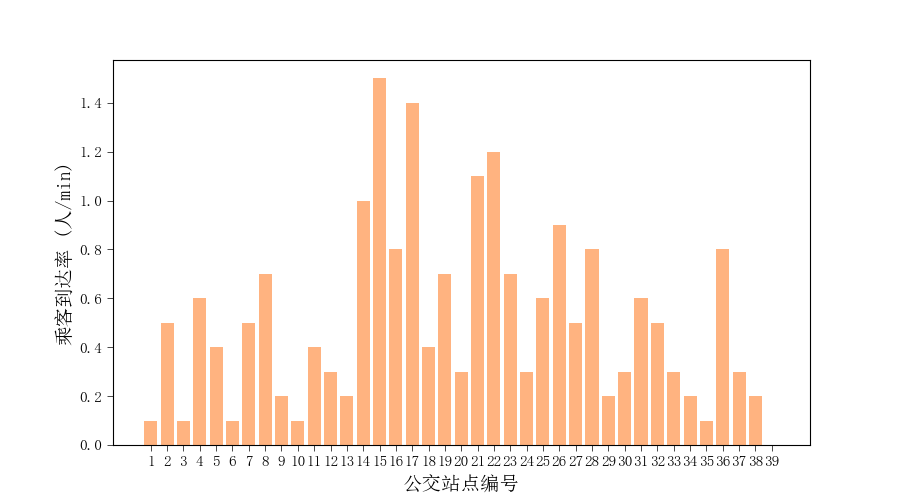
\includegraphics[width=1.\linewidth]{figures/单线公交站点乘客到达率.png}
    \caption{T34公交线路站点乘客到达率}
    \label{fig:T34公交站点乘客到达率}
\end{figure}
\subsection{实验设置}
（1）公交驻站设置

本节采用的线行线路公交系统，线路上发出的第一辆公交车$b_{1}$不进行驻站控制，线路上运行的
所有公交车在第一个公交站站点$s_1$和最后一个公交站点$s_{39}$不进行驻站控制。公交在站点的
最大驻站时间$\triangle T$的大小与本章4.1节采用一样的取值，为180 s，同样的，当驻站时间小于30 s
时忽略不计，视公交在站点不进行驻站控制。

（2）每位乘客登上车辆的时间$t_b$和下车时间$t_a$仍然于第3章取一样的值，分别为3 s/人和1.8 s/人。
每位乘客的下车站点在其上车站点后的其他公交站中随机选择，公交运行到最后一个站点时，车上的所有
乘客全部下车，公交完成行程离开线路。

（3）在公交系统运行过程中，当公交站点第一次车辆到站时，公交站点累积乘客到站的时间$T$为6 min。

\subsection{基准策略模型与评价指标}
为了验证模型的有效性，本节选取几个基准策略与所提出的基于改进MAPPO算法模型进行对比。
选取的对比策略模型如下表\ref{tab4-4}所示。

% （1）无控制策略（NH）

% 即在公交系统运行过程中不进行任何干预

% （2）基于固定车头时距的驻站控制策略（HH）

% 根据公交实际车头时距与计划的车头时距的偏差决定是否驻站控制，本章中计划车头时距H取值为6 min。

% （3）基于前向车头时距的驻站控制策略（FH）

% 该控制策略是Daganzo\cite{daganzo2009headway}等人提出来的，驻站时间由
% th = max\{ 0,\overline{d}+g(H_0 - h^-) \} 决定，

\begin{table}[!ht]
\centering
\caption{基准策略模型}
% \resizebox{\textwidth}{!}{
\label{tab4-4}
\begin{tabular}{>{\centering\arraybackslash}m{4.5cm} >{\raggedright\arraybackslash}m{8cm}}
\toprule
\textbf{策略} & \textbf{说明}\\
\midrule
无控制策略（NH） & 在公交系统运行过程中不进行任何干预\\
基于固定车头时距的驻站控制策略（HH）& 根据公交实际车头时距与计划的车头时距的偏差决定
是否进行驻站控制，驻站时间$th=H_0-h^-$，本节中的计划车头时距$H_0$取6 min\\
基于前向车头时距的驻站控制策略（FH）\cite{daganzo2009headway} &  驻站控制时间
$th = max\{ 0,\overline{d}+(\alpha + \beta )(H_0 - h^-) \} $，其中，$H_0$是计划车头时距；
参数$\alpha \in (0,1)$是基础控制灵敏度参数：调整车头时距偏差的强度；
参数$\beta $是吸引参数：单位车头时距偏差导致的额外乘客延误（与需求正相关），取值范围为0.01至1之间；
$ g = \alpha + \beta $为总控制灵敏度参数，需满足$ \beta \leq  g \leq  1 + \beta$；
参数$\overline{d} $为系统性松弛时间，确保驻站时间非负，
需满足$ \overline{d} \geq 3 (\alpha + \beta)\sigma $，$\sigma $为车头时距标准差。
本节中，计划车头时距$H_0$取值为6 min ，
参考论文中的取值，$\alpha$取值为0.2以平衡稳定性与响应速度，$\beta $取值根据乘客的需求高低在0.1和0.05
之间选择，$h^-$是公交到达站点的时间与前车到达该站点的时间差值\\
基于后向车头时距的驻站控制策略（BH）\cite{xuan2011dynamic} & 驻站控制时间
$th = \beta h^+ = \overline{d} + \beta(h^+ - H_0)$，其中，
$h^+ $表示公交到达站点时与后车的车头时距；$\beta$为控制参数，用于平衡与后车车头时距的偏差，
取值采用文中推荐的0.5来平衡稳定性，$\overline{d}$是站点的松弛时间，$H_0$是计划车头时距\\
基于原始MAPPO算法的驻站控制策略（MAPPO） & 采用原始的MAPPO网络，
不对网络结构进行任何更改，即不特别考虑公交到站异步特性的影响，网络参数的取值与本文
提出的改进的MAPPO算法取值保持一致。\\
\bottomrule
\end{tabular}
% }
\end{table}

本节模型的评价指标的评价指标和本章4.1中相同，同样包含四个指标：平均驻站时间（AHT）、
平均等待时间（AWT）、平均旅行时间（ATT）、平均占用离散度（AOD）。
\subsection{模型训练与收敛性分析}
（1）强化学习算法参数取值

基于改进MAPPO强化学习算法超参数的取值如下表\ref{tab4-3}所示。

\begin{table}[!ht]
\centering
\caption{基于改进MAPPO算法超参数的取值}
\label{tab4-3}
\begin{tabular}{>{\centering\arraybackslash}m{1.8cm} >{\centering\arraybackslash}m{3.8cm} >{\centering\arraybackslash}m{1.8cm} >{\centering\arraybackslash}m{1.8cm}}
\toprule
\textbf{参数类别} & \textbf{参数名称} & \textbf{符号} & \textbf{取值} \\
\midrule
\multirow{3}{*}{优化器} & 策略网络学习率 & $\alpha_{\text{Actor}}$ & 1e-4 \\
    & 价值网络学习率 & $\alpha_{\text{Critic}}$ & 1e-4 \\
    & Adam $\epsilon$参数 & $\epsilon$ & 1e-5 \\
\midrule
\multirow{2}{*}{梯度控制} & Actor梯度裁剪阈值 & $c_{\text{Actor}}$ & 15 \\
    & Critic梯度裁剪阈值 & $c_{\text{Critic}}$ & 5 \\
\midrule
\multirow{3}{*}{强化学习} & 折扣因子 & $\gamma$ & 0.9 \\
    & GAE参数 & $\lambda$ & 0.95 \\
    & 裁剪参数 & $\epsilon_{\text{clip}}$ & 0.2 \\
    & 小批量大小 & $B$ & 256 \\
    & 每个小批量的更新次数 & $ k$ &  3 \\
\midrule
网络结构 & 注意力头数 & $K$ & 1 \\
\bottomrule
\end{tabular}
\end{table}

% \begin{table}[!ht]
% \centering
% \caption{基于改进的MAPPO算法超参数的取值}
% \label{tab4-3}
% \begin{tabular}{>{\centering\arraybackslash}m{5.5cm} >{\centering\arraybackslash}m{1.8cm} >{\centering\arraybackslash}m{3.8cm} >{\centering\arraybackslash}m{1.8cm}}
% % \begin{tabular}{cccp{0.1\textwidth}}
% \toprule
% \textbf{参数} & \textbf{取值} &  \textbf{参数} & \textbf{取值}\\
% \midrule
% 策略网络$Actor$的学习率 & 1e-4  &  $Adam$优化器$eps$参数 & 1e-5\\
% 价值网络$Critic$的学习率 & 1e-4  & 折扣因子$\gamma $ & 0.9\\
% 策略网络$Actor$的梯度裁剪阈值 & 15 & $GAE$的参数$\lambda $ & 0.95 \\
% 价值网络$Critic$的梯度裁剪阈值 & 5 & 裁剪参数$ \epsilon $ & 0.2\\
% 策略熵的系数$\beta $ & 0.01  & 小批量大小B & 256 \\
% 每个小批量的更新次数 &  3 & 注意力头数$K$ & 1  \\
% 激活函数负斜率 & 0.2  \\
% \bottomrule
% \end{tabular}
% \end{table}

（2）模型训练结果

本节所提出的公交运行系统中，一个训练回合是指线路上第一辆公交发车开始至最后一辆
公交完成服务后离开线路时为止。
对模型进行300回合的模拟训练。
下图\ref{fig:改进的多智能体强化学习模型在线形公交线路的训练结果}
分别为策略网络（Actor）和评价网络（Critic）经过300模拟回合的训练结果，
从左侧图（a）中可以看出，大约在50个回合后模型趋于收敛，图中的
橙色曲线表示每15个回合训练过程中获得的总奖励的滑动平均值。
右侧图（b）显示的价值网络的均方误差在50回合后降低至较低水平且趋于平稳，
表明价值网络在训练中不断优化，对价值估计的准确性提高，为策略网络学习提供有效反馈。
\captionsetup{justification=centering} % 设置题注内容居中
\begin{figure}[!ht] 
    \centering
    \begin{subfigure}[t]{0.45\textwidth}
        \centering
        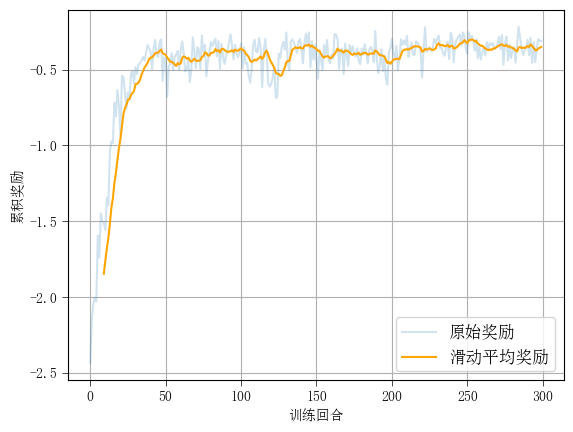
\includegraphics[width=\linewidth]{figures/line累积奖励.png}
        \caption{策略网络每个训练回合的累积奖励}
    \end{subfigure}
    \quad
    \begin{subfigure}[t]{0.45\textwidth}
        \centering
        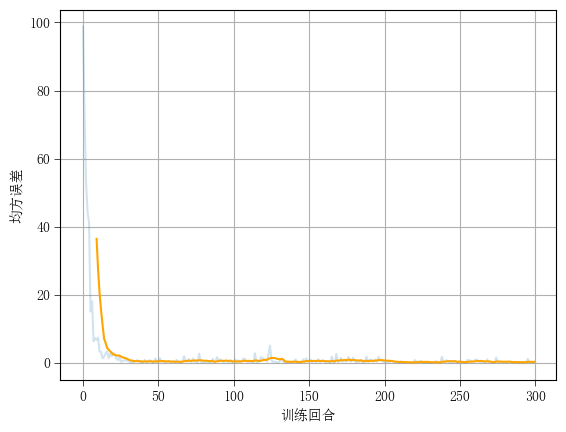
\includegraphics[width=\linewidth]{figures/line_评价网络.png}
        \caption{评价网络的均方误差}
    \end{subfigure}
    \caption{改进MAPPO模型在线形公交线路的训练结果}
    \label{fig:改进的多智能体强化学习模型在线形公交线路的训练结果}
\end{figure}

\subsection{模型验证与性能分析}
在线形公交系统中，所有车辆从发车站点按照发车时刻表依次发车，基于不同的控制策略，公交系统中
车辆的运行轨迹如下图\ref{fig:不同控制策略下线形公交线路的公交运行车辆轨迹}所示，对比不同控制策略下
车辆的运行轨迹可以看出，所提出的策略的有效性。
\captionsetup{justification=centering} 
\begin{figure}[!ht] 
    \centering
    \begin{subfigure}[b]{0.45\textwidth}
        \centering
        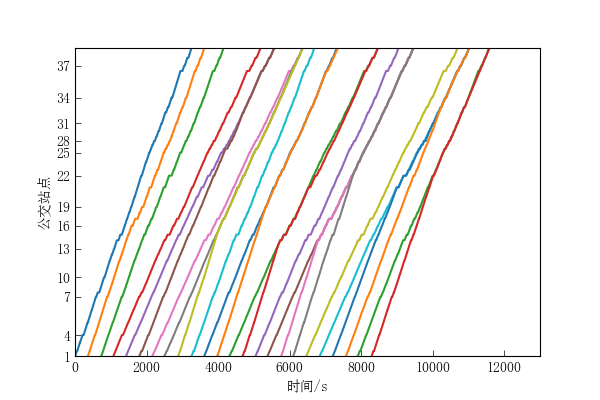
\includegraphics[width=\linewidth]{figures/line_NH车辆轨迹.png}
        \caption{无控制策略（NH）}
    \end{subfigure}
    \quad
    \begin{subfigure}[b]{0.45\textwidth}
        \centering
        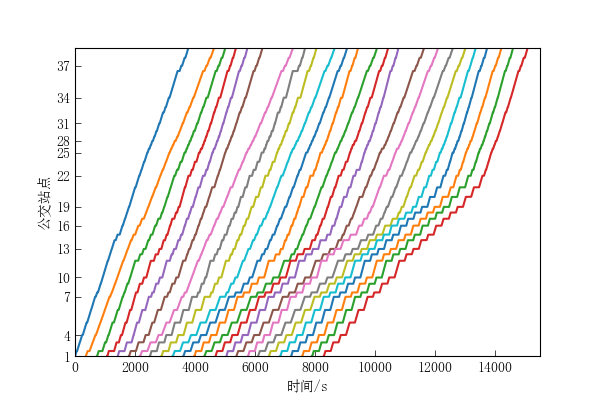
\includegraphics[width=\linewidth]{figures/line_HH车辆轨迹.png}
        \caption{基于固定车头时距的控制策略（HH）}
    \end{subfigure}
    \vskip 10pt % 子图组间垂直间距
    \begin{subfigure}[b]{0.45\textwidth}
        \centering
        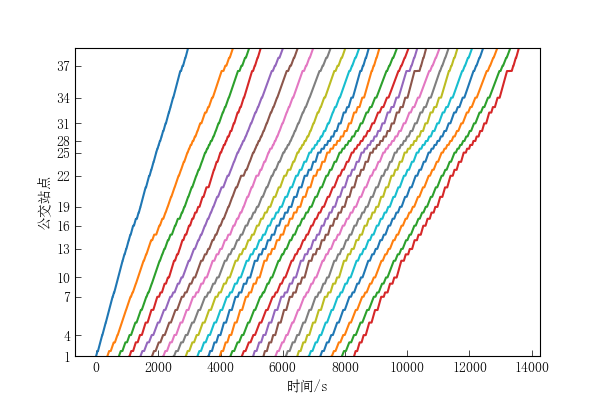
\includegraphics[width=\linewidth]{figures/line_FH车辆轨迹.png}
        \caption{基于前向车头时距的控制策略（FH）}
    \end{subfigure}
    \quad
    \begin{subfigure}[b]{0.45\textwidth}
        \centering
        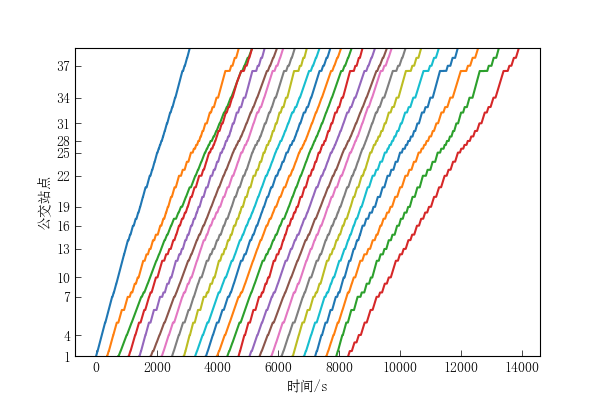
\includegraphics[width=\linewidth]{figures/line_BH车辆轨迹.png}
        \caption{基于后向车头时距的控制策略（BH）}
    \end{subfigure}
    \vskip 10pt % 子图组间垂直间距
    \begin{subfigure}[b]{0.45\textwidth}
        \centering
        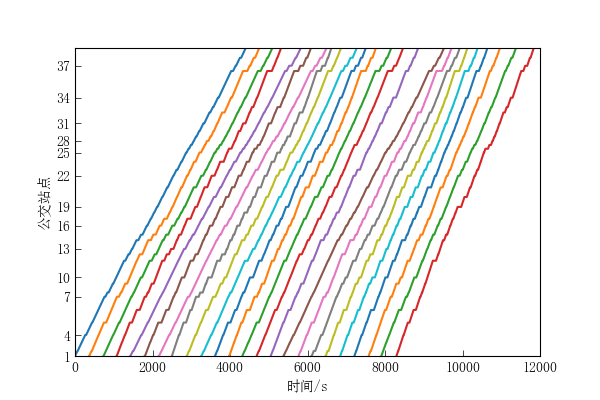
\includegraphics[width=\linewidth]{figures/line_mappo车辆轨迹.png}
        \caption{基于MAPPO算法的控制策略}
    \end{subfigure}
    \quad
    \begin{subfigure}[b]{0.45\textwidth}
        \centering
        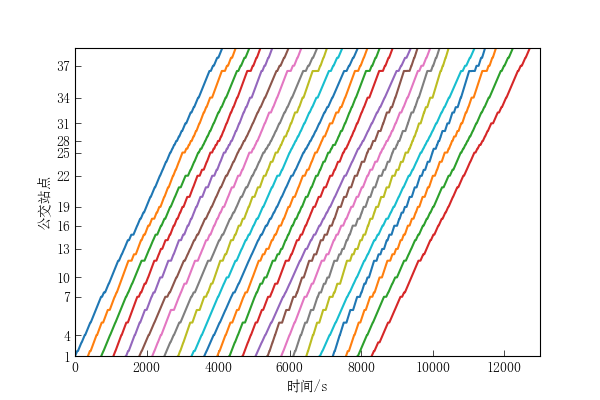
\includegraphics[width=\linewidth]{figures/line_改进的mappo车辆轨迹.png}
        \caption{基于改进的MAPPO算法的控制策略}
    \end{subfigure}
    \caption{不同控制策略下的公交运行车辆轨迹}
    \label{fig:不同控制策略下线形公交线路的公交运行车辆轨迹}
\end{figure}

图\ref{fig:不同控制策略下线形公交线路的公交运行车辆轨迹}（a）显示，无控制（NH）的情况下，
线路上车辆的车头时距严重不均衡，
公交串车情况最严重。串车尤其发生在线路下游站点，因为在线路的上游，车
辆按照发车时刻表发车，车头时距比较均衡，在运行中存在的不确定性会造成车辆的延误，
延误会随着运行时间的增加不断积累，
导致在下游站点出现车辆串在一起。

从图\ref{fig:不同控制策略下线形公交线路的公交运行车辆轨迹}（b）可以看出，基于规则的
固定车头时距（HH）的控制模型，可以缓解公交串车的发生，通过在上游站点对车辆的控制干预，
使得线路上车辆在下游站点的车头时距较为均衡。
从图\ref{fig:不同控制策略下线形公交线路的公交运行车辆轨迹}（c）基于前向车头时距（FH）的控制模型
同样在一定程度可以缓解公交串车的发生，但是对于车头时距均衡的改善不明显。
图\ref{fig:不同控制策略下线形公交线路的公交运行车辆轨迹}（d）基于后向车头时距（BH）的控制模型，
同样可以减少线路上串车的发生，从图中可以看出，线路中仍然存在部分串车现象，车头时距
不稳定现象主要出现在下游站点和后发出的公交车辆之间。由于策略设定，线路上运行的最后一辆车
没有后向车辆，进行驻站决策时，其后向车头时距视为计划车头时距，这会对决策产生影响，
对于前车来说，后向车头的时距又
会影响其驻站决策，这种影响逐渐向前车传播，这是可能是导致后发出车辆见车头时距偏差较大的原因。

图\ref{fig:不同控制策略下线形公交线路的公交运行车辆轨迹}（e）和（f）是基于强化学习的
驻站控制策略下的车辆轨迹，从图中可以看出，策略对于缓解线路上公交串车的出现以及
均衡车头时距方面均有良好的改善，因此在保持车辆车头时距的规律性和减少串车发生方面，
基于强化学习的控制方法表现最佳。对比图（e）和（f）可知，相比于基于原始MAPPO算法控制策略，
本文提出的基于改进MAPPO算法的控制策略公交系统运行的总时间最少，车头时距也更加均衡。


考虑到公交串车的不确定性，为了保证实验结果的稳定性，在不同的控制策略下分别进行
20次运行控制模拟，取不同控制策略下的平均值进行比较分析。

\captionsetup{justification=centering} 
\begin{figure}[!ht] 
    \centering
    \begin{subfigure}[b]{0.45\textwidth}
        \centering
        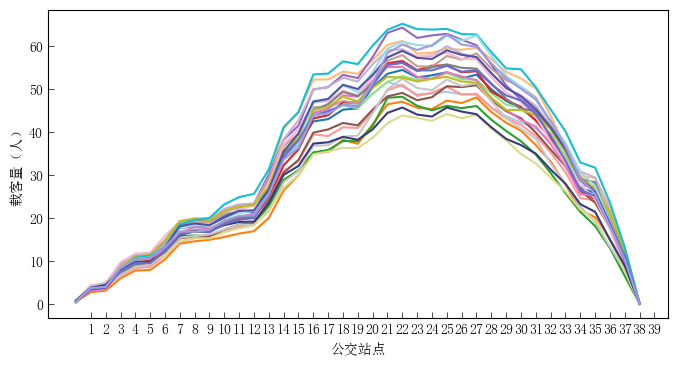
\includegraphics[width=\linewidth]{figures/line_NH载客量.png}
        \caption{无控制策略（NH）}
    \end{subfigure}
    \quad
    \begin{subfigure}[b]{0.45\textwidth}
        \centering
        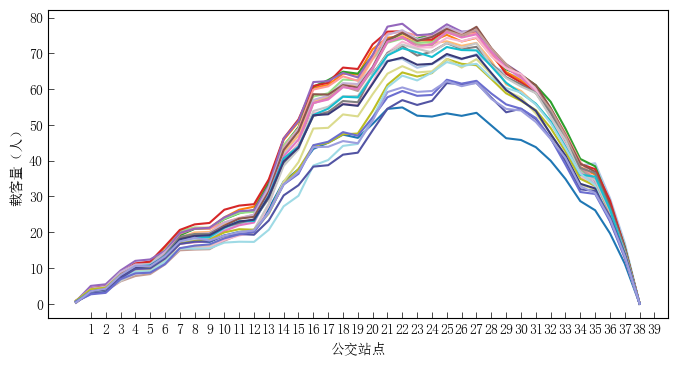
\includegraphics[width=\linewidth]{figures/line_HH载客量.png}
        \caption{基于固定车头时距的控制策略（HH）}
    \end{subfigure}
    \vskip 10pt % 子图组间垂直间距
    \begin{subfigure}[b]{0.45\textwidth}
        \centering
        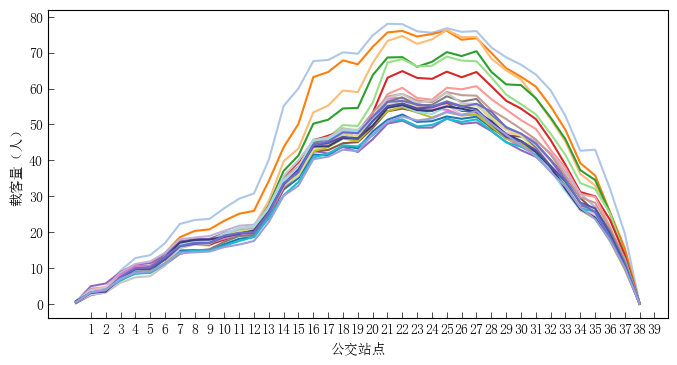
\includegraphics[width=\linewidth]{figures/line_FH载客量.png}
        \caption{基于前向车头时距的控制策略（FH）}
    \end{subfigure}
    \quad
    \begin{subfigure}[b]{0.45\textwidth}
        \centering
        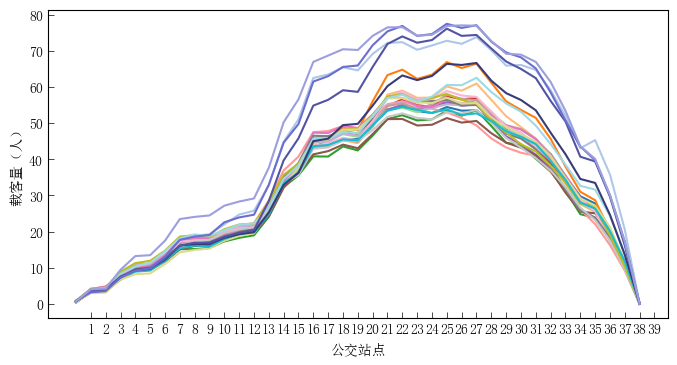
\includegraphics[width=\linewidth]{figures/line_BH载客量.png}
        \caption{基于后向车头时距的控制策略（BH）}
    \end{subfigure}
    \vskip 10pt % 子图组间垂直间距
    \begin{subfigure}[b]{0.45\textwidth}
        \centering
        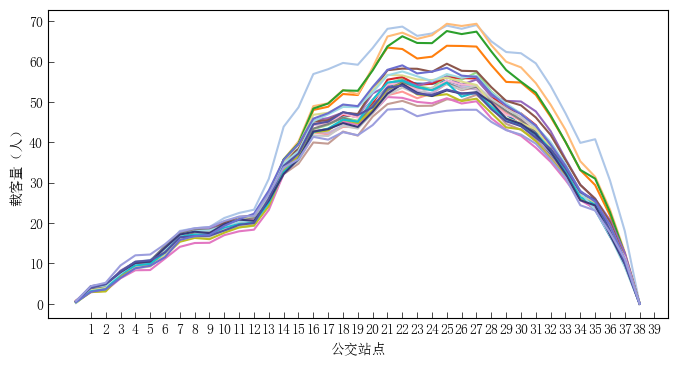
\includegraphics[width=\linewidth]{figures/line_mappo载客量.png}
        \caption{基于MAPPO算法的控制策略}
    \end{subfigure}
    \quad
    \begin{subfigure}[b]{0.45\textwidth}
        \centering
        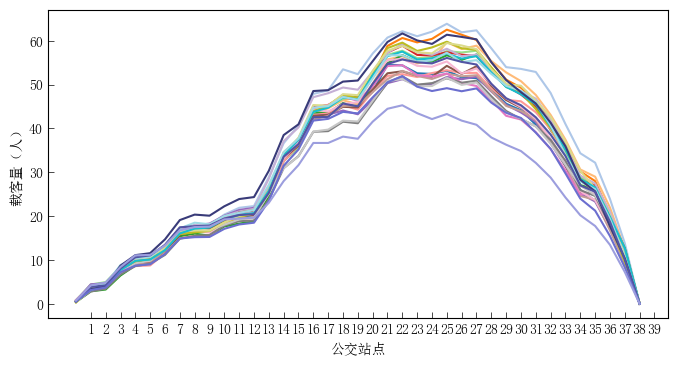
\includegraphics[width=\linewidth]{figures/line_amappo_载客量.png}
        \caption{基于改进MAPPO算法的控制策略}
    \end{subfigure}
    \caption{不同控制策略下各公交在站点的载客量}
    \label{fig:不同控制策略下各公交在站点的载客量}
\end{figure}


下图\ref{fig:不同控制策略下各公交在站点的载客量}展示了在不同控制策略下，系统中
每辆公交车在每个站点的公交载客量。从图中可以看出，相较于无控制情况下，其他控制
策略对于均衡线路上公交的载客量都有一定改善。其中，
基于后向车头时距（BH）的控制策略相对来说在该指标上表现较差，这由于基于该策略的控制，
对车辆车头时距的规律性改善不明显，从而使公交载客量的离散度较大。
图\ref{fig:不同控制策略下各公交在站点的载客量}（b）
相比之下载客量均衡性有一定改善，这与上图呈现出的该控制策略下车辆车头时距较均衡表现一致。
图\ref{fig:不同控制策略下各公交在站点的载客量}（e）和（f）车辆的载客量均衡度有了较大程度的改善，
基于改进MAPPO算法的控制策略下，不同车辆间载客量的变化程度更小，载客量更均匀。


上述从微观层面进行了模型对比分析，接下来，从公交系统的宏观层面对模型进一步对比评价。
下图\ref{fig:站点乘客平均等待时间AWT}（a）展示了在不同控制策略下，每个站点乘客的平均
等待时间（AWT），图中不同颜色的数据条长度表示不同策略下相应站点的乘客平均等待时间，从图中可以
直观的看出，蓝色柱形条和橙色柱形条相比于其他长度更短，表明在这两个策略（基于强化学习）
下乘客的等待时间更短，也显示出了强化学习策略优于其他基于规则和基于优化模型的控制策略。

为了更直观的比较改进MAPPO算法控制模型与原始MAPPO算法控制模型的性能，下图\ref{fig:站点乘客平均等待时间AWT}（b）
展示了两种策略下站点乘客的平均等待时间，可以看出在大部分站点，改进后的模型乘客在站点的等待
时间均下降了。
\captionsetup{justification=centering} % 设置题注内容居中
\begin{figure}[!ht] 
    \centering
    \begin{subfigure}[t]{0.48\textwidth}
        \centering
        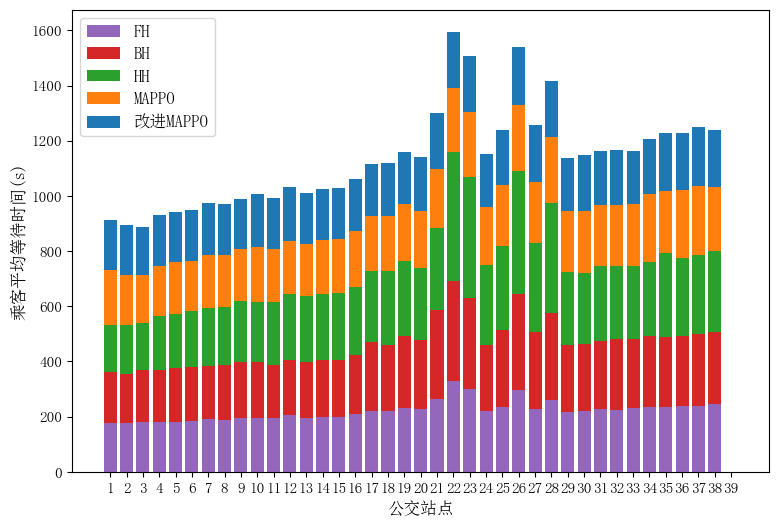
\includegraphics[width=\linewidth]{figures/line_awt.png}
        \caption{不同控制策略的平均等待时间}
    \end{subfigure}
    \quad
    \begin{subfigure}[t]{0.48\textwidth}
        \centering
        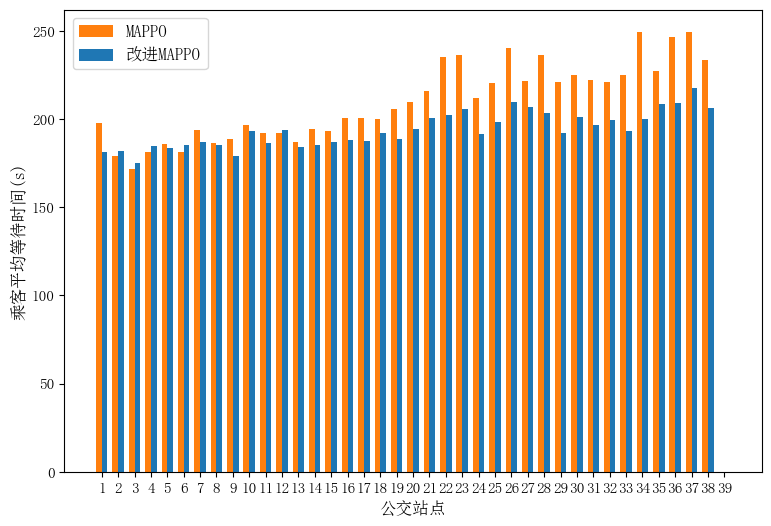
\includegraphics[width=\linewidth]{figures/line_awt对比.png}
        \caption{强化学习策略的平均等待时间}
    \end{subfigure}
    \caption{站点乘客平均等待时间AWT}
    \label{fig:站点乘客平均等待时间AWT}
\end{figure}

% \begin{figure}[!ht]
%     \centering
%     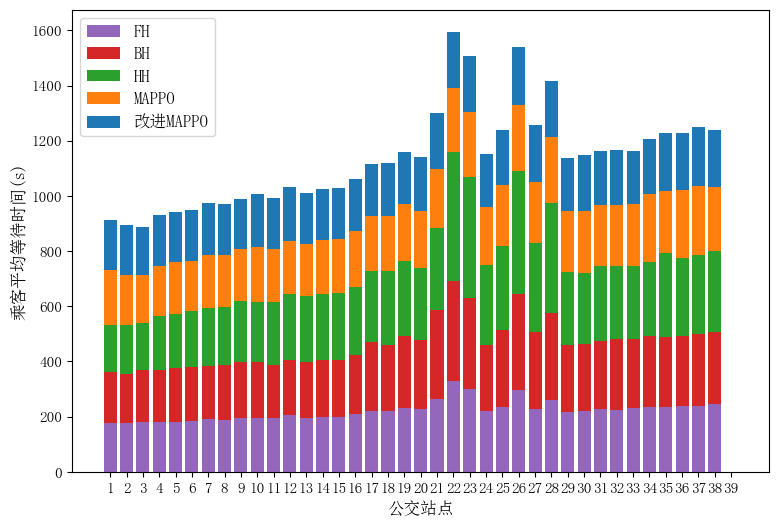
\includegraphics[width=0.7\linewidth]{figures/line_awt.png}
%     \caption{不同控制策略的平均等待时间}
%     \label{fig:不同控制策略的平均等待时间}
% \end{figure}


% \begin{figure}[!ht]
%     \centering
%     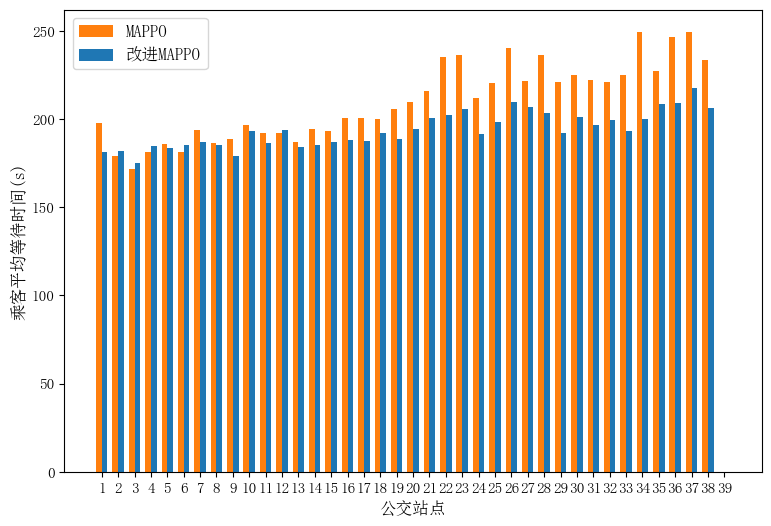
\includegraphics[width=0.7\linewidth]{figures/line_awt对比.png}
%     \caption{强化学习策略的平均等待时间}
%     \label{fig:强化学习策略的平均等待时间}
% \end{figure}

下图\ref{fig:站点车辆平均驻站时间AHT}（a）是不同控制策略下，每个公交站点车辆的平均驻站
时间（AHT）。从图中可以看出，在下游站点基于固定车头时距的控制策略（HH）的驻站控制
干预最小，这与上图\ref{fig:不同控制策略下线形公交线路的公交运行车辆轨迹}（b）车辆轨迹
呈现的结果相同，通过上游站点的驻站干预，保持了车头时距的相对稳定，减小了在下游站点的
干预程度。图中的红色数据条表示基于后向车头时距的控制策略（BH），其驻站时间相对
与基于前向车头时距（FH）和基于固定车头时距（HH）的控制策略更小。
基于强化学习的驻站控制策略，公交在站点的平均驻站时间
更短，明显优于其他控制策略，更低的驻站控制时间表征了控制策略
对于公交系统运行的更小干预程度。

\captionsetup{justification=centering} % 设置题注内容居中
\begin{figure}[!ht] 
    \centering
    \begin{subfigure}[t]{0.48\textwidth}
        \centering
        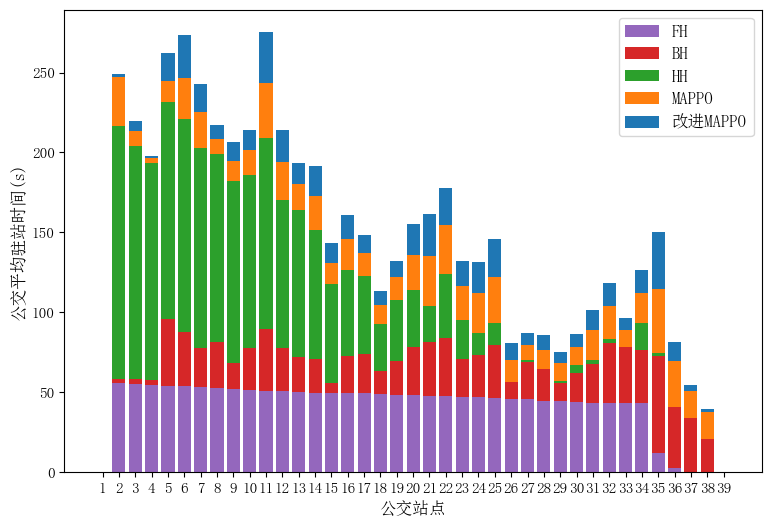
\includegraphics[width=\linewidth]{figures/line_ahr.png}
        \caption{不同控制策略的平均驻站时间}
    \end{subfigure}
    \quad
    \begin{subfigure}[t]{0.48\textwidth}
        \centering
        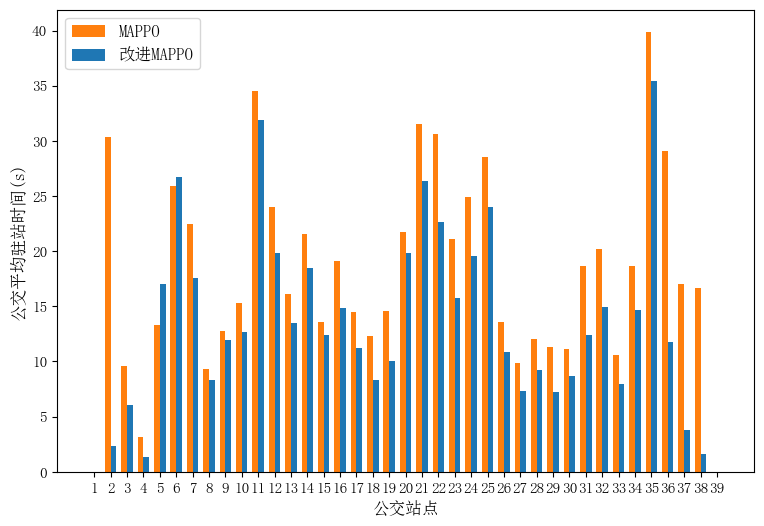
\includegraphics[width=\linewidth]{figures/line_aht对比.png}
        \caption{强化学习策略的平均驻站时间}
    \end{subfigure}
    \caption{站点车辆平均驻站时间AHT}
    \label{fig:站点车辆平均驻站时间AHT}
\end{figure}

图\ref{fig:站点车辆平均驻站时间AHT}（b）对比了两种强化学习策略下公交在站点的驻站时间，
在大部分站点，基于改进MAPPO算法的公交驻站时间都小于基于原始MAPPO算法的驻站
时间，显示出了改进后模型的优势。这也证明在原始MAPPO算法中引入图注意力网络（Graph Attention Network，GAT）可以很好的
量化其他智能体异步到站控制动作的影响，使得智能体可以更好的做出决策。


\captionsetup{justification=centering} % 设置题注内容居中
\begin{figure}[!ht] 
    \centering
    \begin{subfigure}[t]{0.48\textwidth}
        \centering
        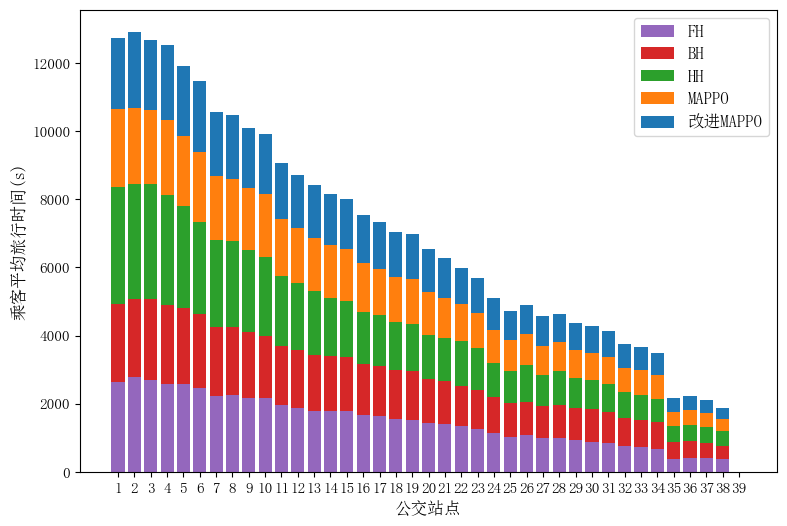
\includegraphics[width=\linewidth]{figures/line_att.png}
        \caption{不同控制策略的平均旅行时间}
    \end{subfigure}
    \quad
    \begin{subfigure}[t]{0.48\textwidth}
        \centering
        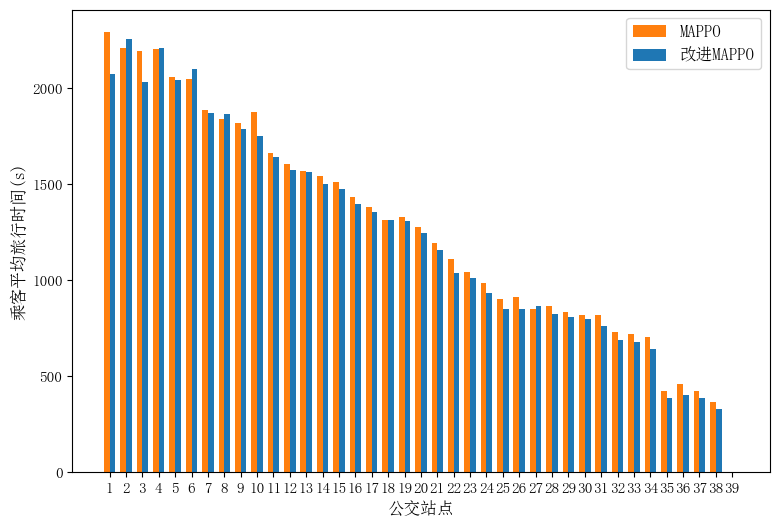
\includegraphics[width=\linewidth]{figures/line_att对比.png}
        \caption{强化学习策略的平均旅行时间}
    \end{subfigure}
    \caption{站点乘客平均时间旅行ATT}
    \label{fig:站点乘客平均旅行时间ATT}
\end{figure}



图\ref{fig:站点乘客平均旅行时间ATT}（a）是不同控制策略下在每个公交站点登上车辆的
的乘客的平均旅行时间（表示乘客的出行时间，从乘客到达站点开始至结束行程离开站点的总用时）。
图中可以看出，不同的策略
都呈现出来了上游站点的平均旅行时间（ATT）大于下游站点，这是由于相比于下游站点，
在上游站点上车的乘客下车站点的选择更多，导致可能的出行时间更长。
同样可以看出，蓝色数据条和橙色数据条相比于其他长度更短，
证明了基于强化学习的控制策略在该指标上也表现更优。

为了更直观的对比，图\ref{fig:站点乘客平均旅行时间ATT}（b）展示了两种强化学习控制模型在该指标（ATT）
上的表现性能比较，总体上本文提出的基于改进MAPPO算法的控制模型表现更好。

\captionsetup{justification=centering} % 设置题注内容居中
\begin{figure}[!ht] 
    \centering
    \begin{subfigure}[t]{0.48\textwidth}
        \centering
        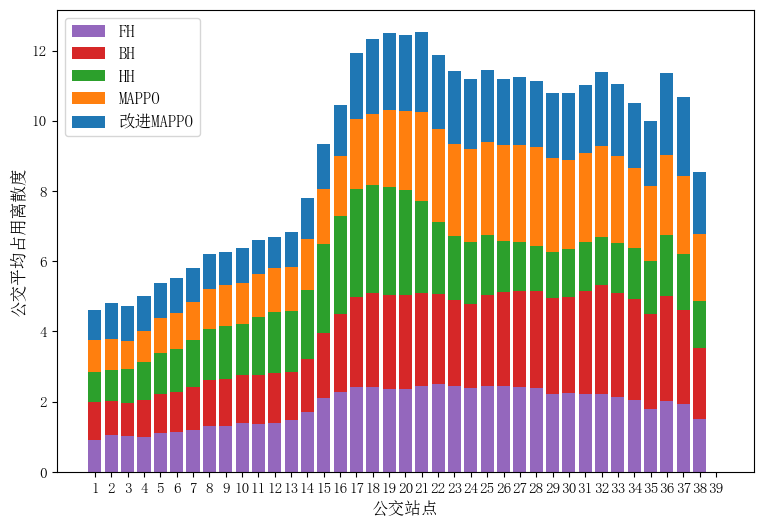
\includegraphics[width=\linewidth]{figures/line_aod.png}
        \caption{不同控制策略的车辆平均载客量离散度}
    \end{subfigure}
    \quad
    \begin{subfigure}[t]{0.48\textwidth}
        \centering
        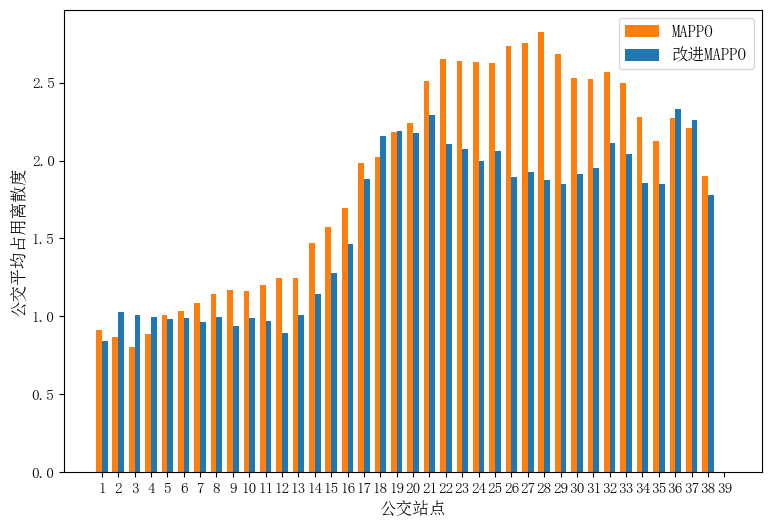
\includegraphics[width=\linewidth]{figures/line_aod_对比.png}
        \caption{强化学习策略的车辆平均载客量离散度}
    \end{subfigure}
    \caption{站点车辆平均载客量离散度AOD}
    \label{fig:站点车辆平均载客量离散度AOD}
\end{figure}

图\ref{fig:站点车辆平均载客量离散度AOD}（a）是不同控制策略下在每个公交
车辆在离开站点时的车辆载客离散度（AOD值越大，表明车上乘客数量越不均衡）。图中可以看出，
在下游站点基于固定车头时距的控制策略（HH）在该指标上表现最好，如图中的绿色数据条所示，因为该策略在公交上游站点进行了大量的控制
干预，使得线路上的公交在下游站点车头时距
保持良好的规律性，从而车辆的载客量较均衡。

除此之外，仍然是基于强化学习的控制策略在该指标上表现更好。
图\ref{fig:站点车辆平均载客量离散度AOD}（b）可以更直观的看出两种强化学习的策略在
该指标上的表现，改进后的MAPPO算法在大部分站点的车辆载客离散度明显优于原始MAPPO算法
控制策略。


在线性公交线路中，不同控制策略在运行完一个回合（即公交线路上从第一辆车发车开始到最后一辆车
完成服务离开线路为止）乘客的平均等待时间（AWT）、公交在站点的平均驻站时间（AHT）、
乘客的平均旅行时间（ATT）
及公交车辆的载客离散度（AOD）四项指标的性能对比如下表\ref{tab4-5}所示，
可以看出，本文所提出的驻站控制模型在各项指标上均表现较好。

\begin{table}[!ht]
\centering
\caption{不同控制策略下的评价指标对比}
\label{tab4-5}
\begin{tabular}{>{\centering\arraybackslash}m{3cm} >{\centering\arraybackslash}m{2.4cm} >{\centering\arraybackslash}m{2.4cm} >{\centering\arraybackslash}m{2.4cm} >{\centering\arraybackslash}m{2.4cm}}
\toprule
\textbf{控制策略} & \textbf{平均等待时间(s)} &  \textbf{平均驻站时间(s)} & \textbf{平均旅行时间(s)} & \textbf{平均车辆占用离散度}\\
\midrule
NH & 289  & 0 & 1278 & 7.0\\
HH & 261  & 51  & 1553 & 1.7\\
FH & 215 & 42 & 1467 & 1.8 \\
BH & 235 & 24 & 1344  & 2.0 \\
MAPPO & 204  & 18 & 1260 & 1.8 \\
改进的MAPPO &  \textbf{188} & \textbf{13} & \textbf{1223} & \textbf{1.6}  \\
\bottomrule
\end{tabular}
\end{table}

相比于无控制模型（NH），其他控制策略在乘客的平均等待时间（AWT）和车辆的平均占用离散度（AOD）
两个指标上性能都有提升，在一定程度上减少了乘客的平均等待时间，均衡了系统中
车辆的载客量，提升了资源利用率及乘车的舒适性；但基于固定车头时距的控制策略（HH）、
基于前向车头时距（FH）和后向车头时距（BH）的控制策略
相比于无控制乘客的平均旅行时间增加了，这主要是由于这些控制策略增加的公交驻站时间导致的。

具体来说，强化学习方法在各项指标上表现更好。其中，本文所提出的基于改进MAPPO算法
的驻站控制模型相比于无控制模型（NH）、基于固定车头时距的控制模型（HH）、基于前向车头时距（FH）和
后向车头时距（BH）的控制模型在乘客平均等待时间（AWT）的指标上分别减少了 34.95\%、27.97\%、12.56\%、
20.00\%，
主要原因是强化学习方法能实时感知交通状态、客流信息等环境变化，动态调整驻站时间，
可以更好地适应实际情况，减少因不合理驻站导致的乘客长时间等待。
相比原始MAPPO算法模型在该指标上性能提升了7.84\%，原因在于，本文所提出的算法能更好捕捉
异步到站信息和量化智能体间的影响，从而作出更优的驻站决策；
在乘客平均旅行时间（ATT）方面，相比于其他策略分别减少了
4.3\%、21.25\%、16.63\%、8.99\%，相比原始MAPPO算法模型在该指标上性能提升了2.94\%，
即时增加了额外的驻站控制干预，乘客的平均旅行时间相对于无控制情况下还是降低了。
相比于强化学习的控制策略，其他控制策略进行驻站决策时往往只考虑短期影响，单控制点驻站时间过长，
导致延误积累增加乘客的旅行时间，导致这些控制策略下（HH、FH、BH）的乘客平均旅行时间相比于
无控制策略延长了。
在车辆的平均占用离散度（AOD）指标上，分别减少了 77.14\%、5.88\%、11.11\%、20.0\%，
相比原始MAPPO算法模型在该指标上性能提升了11.11\%；
在车辆的平均驻站时间（AHT）指标上，
相比于基于固定车头时距的控制模型（HH）、基于前向车头时距（FH）和
后向车头时距（BH）的控制模型分别减少了 74.51\%、69.05\%、45.83\% ，相比原始
MAPPO算法模型在该指标上性能提升了27.78\%。


\section{本章小结}

本章基于前文提出的改进多智能体近端策略优化（改进MAPPO）公交驻站防串车控制方法，
通过单向环形公交线路仿真实验和成都T34路公交线路真实场景
展开实证分析，系统评估了算法的有效性与应用潜力。从算法收敛性、
公交串车缓解情况、乘客出行效率及公交运行效率和服务质量等维度综合评估其性能优势。
具体而言，设计单向环形公交基准实验场景（均匀站点分布、等距站间距、恒定运行速度、无
外部交通干扰），验证了算法在理想环境下的性能。
接着，选取成都市T34路公交线路（全长21千米，39个站点）作为实证对象，
构建融合真实乘客需求及随机路况干扰的高保真仿真环境。
通过分析算法训练结果，并选取多维度评价指标对比分析，数值结果表明，
改进MAPPO算法通过动态协同决策机制，可有效应对复杂交通环境中的不确定因素，
有效缓解公交串车现象，同时降低了乘客的出行时间成本，提高了公交运行效率和服务质量。

% 基于线路上行方向的GPS轨迹数据、站点分布及发车时刻表等多源信息
% 实验结果表明，改进MAPPO算法
% 收敛速度较快，

% 本章在前一章研究的基础上进行了拓展与深化，
% 将研究视角从相对简化的场景转向更贴近现实的公交运行情境。
% 具体而言，充分考量了公交运行过程中诸如交通流量变化、路况差异等干扰因素，同时纳入了发车间隔
% 以及站点分布等关键要素。为使模型构建更具可行性与可操作性，做出了一系列合理假设，
% 包括公交车辆性能同质、最大载客量保持一致以及乘客候车耐心相同等，
% 从而对实际复杂的公交运行状况进行了适度简化。
% 本章以成都市 T34 路公交线路为具体研究对象，通过对公交车辆 GPS 轨迹数据、站点 GPS 数据以及线路信息等
% 多源数据的处理，梳理出了 T34 路公交上行方向的关键信息，
% 如线路的总长度、站点的具体数量、相邻站点之间的距离、研究时段内的发车时刻表、
% 平均运行速度以及速度方差等，为后续的研究提供了数据支撑。
% 基于上述的数据基础，进一步进行了仿真模拟设置，并对基于改进的 MAPPO 算法的模型进行训练。
% 为了验证模型的有效性与优越性，将所构建的模型与多个基准模型进行了全面对比。
% 从微观和宏观层面多维度进行了对比分析，展示出本文所提出的基于改进的 MAPPO 算法的驻站控制模
% 型相较于其他模型的显著优势。

% 综上所述，本章通过理论建模和实际数据验证，充分证明了基于改
% 进的 MAPPO 算法的公交驻站控制策略在提高公交运行效率和服务质量方面的有效性和优越性。


\chapter{结论与展望}
\section{研究工作总结}
本文在人工智能体、大数据以及智能网联公交系统环境下，
针对常规公交运行中由于外部干扰导致车头时距不稳定而产生的串车问题，探究了多智能体
强化学习在公交驻站控制策略中的应用，创新性地提出了基于改进多智能体近端策略优
化（改进MAPPO）算法的动态驻站控制模型。通过理论建模、模型训练与实例分析相结合，
系统性地证明本文所提出的模型在多车协同控制中异步决策问题的优势，
结果表明该模型在保持车头时距稳定、减少公交串车的发生、减少乘客等待时间及
提升公交运行效率和服务质量方面具有显著优势。
主要研究结论归纳如下：

（1）本文基于马尔可夫博弈（Markov Game, MG）理论，描述了多个智能体在环境中交互的动态过程，
在马尔可夫博弈过程中，状态转移依赖于所有智能体的联合动作，但在公交驻站控制中，由于系统中
公交到站的异步特征，使得状态转移变得不准确，因此本文进行了独立性假设，同时提出解决方法
有效考虑其他智能体的影响，基于此，本文将公交动态协同驻站控制建模为了考虑异步特性的
多智能体强化学习模型。

（2）本文在考虑公交到站异步特性的基础上，基于公交异步到站的运行过程构建了事件图（Event Graph）网络，
以多智能体近端策略优化（Multi-Agent Proximal Policy Optimization, MAPPO）算法为基础，
在策略网络中引入图注意力网络（Graph Attention Network, GAT）来学习图结构信息，
从而来量化其他智能体的到站控制动作对目标智能体的影响，使策略网络能够更好的
进行控制决策，构建了基于改进MAPPO算法的公交驻站控制模型。通过设计单向环形公交线路
运行场景，对模型进行训练，得到控制后的公交系统运行结果，通过与基准模型的对比分析和评价指标
的评估，验证了所提出的模型的有效性。

（3）为了进一步验证模型的有效性和实用性，将模型的应用场景进一步扩展至常规公交线路，
考虑了更现实的情况，包括站点分布、公交运行速度以及运行过程中的存在的干扰等，
将单向公交运行系统建模为多智能体强化学习模型，进行了状态空间、动作空间、
奖励函数、状态转移函数的设计，模型的优化目标是在保持系统车头时距均衡的同时，尽可能减少乘客
在站点的等待时间成本。将该控制模型应用于成都市T34公交线路，结果表明，本文所提出的模型
在保持车头时距的稳定性、减少公交串车、降低乘客出行的时间成本以及提高公交资源的利用率方面
表现出良好性能。

\section{主要创新点}

（1）基于图注意力网络的多智能体异步决策建模方法

针对公交异步到站导致的异步控制问题，提出一种改进的多智能体近端策略优化
（Multi-Agent Proximal Policy Optimization）算法：通过事件图（Event Graph）动态表征车辆到站事件的异步依赖关系，
在策略网络（Actor）中引入图注意力网络（Graph Attention Network），量化车辆间异步到站交互影响强度，
提升策略决策的协同性；针对集中式评价网络（Critic）复杂度随车辆数指数增长的问题，采用基于局部观测的价值函数估计，
降低计算开销，增强算法在大规模车队场景下的可扩展性。

（2）融合时空特征的多目标奖励函数设计

针对公交运营中效率与稳定性的平衡难题，本文在强化学习的奖励函数中构建两类核心指标：
以时变乘客等待时间成本量化出行效率，以车头时距均衡性反映运营稳定性。通过设置权重参数实现多目标间的协同优化，
一方面通过保持公交车头时距的稳定减少公交串车的出现，另一方面最小化乘客在站点的等待耗时与整体出行时间，
通过该设计实现公交系统运行效率与乘客体验的协同改善。



% 针对公交运营中效率与稳定性的平衡难题，先前的研究大在奖励函数的设计中，
% 通过设置过度干预惩罚项间接降低驻站控制对乘客出行效率的影响，本文设计了包含均衡公交车头时距、降低乘客等待时间成本的
% 多目标奖励函数，实现多目标协同优化，通过在奖励函数中直接引入乘客的等待时间成本，直接减低
% 控制干预对乘客出行效率的影响。
% （1）构建了面向公交驻站控制的多智能体强化学习模型。
% 通过马尔可夫博弈理论，将公交驻站控制问题建模为多智能体强化学习问题，
% 基于公交运行过程建立了事件图，
% 创新性地在MAPPO算法中引入图注意力网络（Graph Attention Network，GAT）学习事件图结构信息，以此量化智能体间异步到站的
% 影响，从而使策略网络可以做出更优的决策，
% 有效解决了传统方法难以处理车辆到站时间异步性的问题。同时，通过去中心化的设计，
% 可以降低模型的计算复杂度，提升模型的效率，
% 增强模型的可扩展性，能够较好的应对系统中智能体数量的增加。
% 结果表明，本文提出的模型在保持公交系统车头时距稳定性
% 和均衡车辆载客量等方面显著优于传统控制模型。

% （2）在本文提出的基于改进的MAPPO算法的公交驻站控制模型中，设计了融合时空特征的状态表征方法，
% 针对公交运营中效率与稳定性的平衡难题，设计了包含均衡公交车头时距、乘客等待时间成本的多维度
% 奖励函数，通过训练不断调整各项权重，实现多目标协同优化，使模型可以在较小的控制干预下，
% 保持公交车头时距的稳定从而减少串车的发生，同时又能最大程度的减少乘客在站点的等待时间，
% 使乘客的整体出行时间缩短，从而提高公交的服务质量。

\section{研究不足与展望}
本文针对公交串车问题，提出了基于改进的MAPPO算法的强化学习驻站控制模型，但在本文研究结论
的基础上仍然存在一些不足，后续的研究可以从以下几个方面进行优化探索：

（1）多线路共线控制研究：本文的公交的运行场景为单线公交线路，下一步可以考虑拓展至区域公交网络层面，
与单线公交线路相比，城市交通网络中存在更多不确定性，公交发生串车的情况更频繁。
未来可将基于多智能体强化学习的控制策略应用于考虑多条公交线路的交通网络，
研究多线路共线车辆调度与驻站控制的协同优化方法，实现网络级运行效率提升。

（2）多模态控制策略融合：本文只考虑公交驻站控制这一策略，未来可考虑多模态控制策略融合，
如将驻站策略与区间巡航调速、跳站控制等策略动态匹配，
可以构建分层决策框架，
有效提升多控制模式的协同性与动态环境适应性。

（3）考虑公交车辆异质性：当前模型假设公交车辆同质化（如容量、速度等性能参数一致），
未来公交车队可进一步纳入不同容量、性能的车辆，研究异质车辆对控制效果的影响。

（4）权衡算法效率与性能：
本文提出的考虑异步控制的多智能体强化学习算法可以提高性能，但相比于单智能算法在一定程度上
提升了计算成本。值得注意的是，在最新研究表明\cite{xu2025reinforcement}，
单智能体强化学习算法在忽略公交异步到站特性及多车协同交互影响的条件下，
也可有效缓解串车现象，未来可探索基于实时计算资源与控制精度需求的动态权衡机制，
针对低负载场景或计算资源受限条件采用单智能体强化学习算法以保证效率，
而在高峰时段或串车风险突出场景启用多智能体异步控制策略以提升协同性能，
通过构建自适应算法选择框架实现效率与性能的最优平衡。

% （4）权衡算法的效率和性能，本文提出的考虑异步控制的多智能体强化学习算法可以提高性能，但相比于单智能算法在一定程度上
% 提升了算法的计算成本，值得注意的是，在最新研究中，在公交串车的控制中，
% 单智能体强化学习算法在忽略公交异步到站特性及多车协同交互影响的条件下，
% 也可有效缓解串车现象。因此，未来的研究中可以...

% 在战略层进行多控制模式选择，在战术层实施具体控制参数优化，

